\Chapter{Additional Techniques for Solving ODEs}
\label{chap:SingleOdes}

In Chapters~\ref{C:HDS}, \ref{C:LDE}, and \ref{C:LT} we developed analytic 
methods for finding solutions to {\em linear differential equations\/} with 
constant coefficients and with forcing.  In this chapter we show how to find 
closed form solutions to certain types of nonlinear equations as well as to 
certain linear equations with time dependent coefficients.

Most nonlinear differential equations cannot be solved analytically and   
for these equations one has to rely either on advanced theory or on 
numerical methods.  There are, however, specific types of ordinary differential 
equations whose solution by hand is possible.  In this chapter we describe 
several of these types.  In Sections~\ref{sec:VarConstS} and 
\ref{sec:LinInhomSys} we solve forced nonconstant coefficient linear 
differential equations and systems using {\em variation of parameters}.  In 
Section~\ref{S:RO} we show how to solve higher order equations by reduction 
to first order systems and by a variant of variation of parameters called 
{\em reduction of order\/}.  
Sometimes it is possible to transform a nonlinear equation into an equation 
that can be treated by one of the methods mentioned above.  This is 
accomplished by substituting another function for the function $x(t)$ in a suitable way.  {\em Simplifications by substitution\/} are discussed in 
Section~\ref{sec:SBS}.  

The chapter ends with a discussion of two types of 
differential equations whose solutions lie on level curves of a real-valued 
function: nonautonomous {\em exact differential equations\/} and autonomous 
{\em Hamiltonian systems}.  Exact equations are treated in 
Section~\ref{S:exact}.   Hamiltonian systems, which arise naturally in 
mechanical systems, are treated in Section~\ref{sec:HamSys}.  


\Section{Nonconstant Coefficient Linear Equations}
\label{sec:VarConstS}

The simplest nonconstant coefficient homogeneous\index{homogeneous} 
linear differential equation is:
\begin{equation}   \label{eq:linhomo1}
\frac{dx}{dt}  =  a(t)x.
\end{equation}
This equation does not have constant coefficients, since the coefficient 
$a$ depends on $t$.  The equation is linear as linear combinations of 
solutions are solutions.  Note that \Ref{eq:linhomo1} is of the form 
\Ref{eq:ghivp} and can be solved by separation of variables. 
\index{separation of variables}

If $x(t_0)=0$, then $x(t)=0$ is the solution to the initial value problem
\Ref{eq:linhomo1}.
To solve the initial value problem $x(t_0)=x_0$ for \Ref{eq:linhomo1}
when $x_0\neq 0$, we apply the technique of separation of variables to 
this equation, which yields
\[
\ln|x| = H(t) + C,
\]
where $H(t)$ is the definite integral
\begin{equation}   \label{e:H(t)}
H(t)=\int_{t_0}^t a(\tau)d\tau.
\end{equation}
Exponentiation implies that
\[
x(t) = Ke^{H(t)}
\]
for an appropriate scalar $K$.  Indeed, if $x(t_0)=x_0$, then
\[
x_0 = x(t_0) = Ke^{H(t_0)} = Ke^0 = K.
\]
We have shown that the function 
\begin{equation} \label{E:ssv}
x(t) = x_0 e^{H(t)}
\end{equation}
is the unique solution\index{uniqueness of solutions} 
to the initial value problem\index{initial value problem} 
\Ref{eq:linhomo1} where $x(t_0)=x_0$.

\subsubsection*{An Example of a Nonconstant Coefficient Equation}

We illustrate \Ref{E:ssv} by an example. Solve the initial value problem
\[
\begin{array}{rcl}
\dps \frac{dx}{dt} & = & -\dps \frac{x}{t} \\
x(2) & = & 5.
\end{array}
\]
Since $a(t)=-\frac{1}{t}$, we can use \Ref{e:H(t)} to compute
\[
H(t)=-\int_2^t \frac{1}{\tau}d\tau = -\ln t +\ln 2 =
\ln\left(\frac{2}{t}\right).
\]
Then the solution \Ref{E:ssv} is given by
\[
x(t) = 5 e^{\ln(2/t)} = \frac{10}{t}.
\]

\subsection*{The Inhomogeneous Equation}
\index{inhomogeneous}

Next, we consider forced linear differential equations of the type
\begin{equation}   \label{eq:linode1}
\frac{dx}{dt} = a(t)x + g(t),
\end{equation}
where $a$ and $g$ are continuous functions of $t$.  The differential  
equation \Ref{eq:linode1} is homogeneous when $g=0$  and 
\index{homogeneous} inhomogeneous otherwise.  As is always the 
case, we find the general solution\index{general solution} 
to the inhomogeneous equation 
by adding the general solution to the homogeneous equation (that
we can find by separation of variables) to a particular solution to 
the inhomogeneous equation.  

\subsubsection*{Two Examples of Solutions of Inhomogeneous Equations}

(a) Find all solutions of the differential equation
\begin{equation} \label{E:ie1}
\frac{dx}{dt} = 3t^2x + 3t^2.
\end{equation}
By inspection, the constant function $x_p(t)=-1$ is a 
particular solution\index{particular solution} 
of \Ref{E:ie1}. 
Since all solutions of the homogeneous equation are of the form $Ke^{t^3}$
for some real constant $K$, it follows that the general solution of the 
inhomogeneous equation is
\[
x(t) = -1 + Ke^{t^3}.
\]

\noindent (b) Find all solutions of the differential equation
\begin{equation}  \label{E:ie2}
\frac{dx}{dt} = \left(\frac{5}{t}-t\right) x + t^6.
\end{equation}
A calculation shows that $x_p(t)=t^5$ is a particular solution of \Ref{E:ie2}. 
Since all solutions to the homogeneous equation are of the form 
$Kt^5 e^{-t^2/2}$ for some real constant $K$, it follows that the general
solution of the inhomogeneous equation is
\[
x(t) = t^5 + Kt^5 e^{-t^2/2}.
\]

\subsection*{Inhomogeneous Equations and Variation of Parameters}
\index{variation of parameters}

In Examples~\Ref{E:ie1} and \Ref{E:ie2} we guessed or were given a
particular solution\index{particular solution!variation of parameters} 
to the inhomogeneous equation.  Now we discuss 
a method for finding a particular solution to the inhomogeneous
equation \Ref{eq:linode1} when $g(t)$ is a nonzero function.   This 
technique for finding a particular solution is called 
{\em variation of parameters\/}.  

We already know by separation of variables that every solution of the 
{\em homogeneous\/} equation ($g=0$) has the form $Ke^{H(t)}$ where 
$\frac{dH}{dt}=a$.  The idea behind variation of parameters is to
allow $K$ to depend on $t$.    \index{variation of parameters}
More precisely, assume that a solution $x(t)$ has the form
\[
x(t) = c(t)e^{H(t)},
\]
where $c$ is a differentiable function of $t$.  Substituting $x(t)$ in 
\Ref{eq:linode1}, using the product rule for differentiation and suppressing
the explicit dependence of functions on $t$, leads to the identity
\[
\frac{dc}{dt}e^{H}+ce^{H}a =  ace^{H}+g,
\]
which simplifies to
\[
\frac{dc}{dt} = ge^{-H}.
\]
This last equation may be solved for $c(t)$ by integration, obtaining
\begin{equation}   \label{eq:c(t)}
c(t) = \int g(\tau)e^{-H(\tau)}d\tau.
\end{equation}
Uniqueness of solutions\index{uniqueness of solutions} to initial 
value problems implies the main result of this section.

\begin{thm}[Variation of Parameters]  \label{thm:varpar}
\index{variation of parameters}
The unique solution to the initial value problem
\index{variation of parameters!initial value problem}
\[
\begin{array}{rcl}
\dps \frac{dx}{dt} & = & a(t)x+g(t) \\
x(t_0) & = & x_0.
\end{array}
\]
is
\[
x(t) = c(t)e^{H(t)},
\]
where 
\[
H(t)=\int_{t_0}^t a(\tau)d\tau \AND
c(t)=\int_{t_0}^t g(\tau)e^{-H(\tau)}d\tau + x_0.
\]
\end{thm} \index{variation of parameters}


\subsubsection*{Two Examples of Variation of Parameters}

(a)   Solve the initial value problem
\begin{equation} \label{e:solntheq}
\begin{array}{rcl}
\dps \frac{dx}{dt} & = & -\dps \frac{x}{t} + \frac{2}{t^4}\\
x(1) & = & 0.
\end{array}
\end{equation}
Compute
\[
H(t)= -\int_1^t\frac{1}{\tau}d\tau = -\ln t +\ln 1 = -\ln t.
\]
Hence 
\[
c(t)=\int_1^t \frac{2}{\tau^4}e^{\ln\tau}d\tau + 0
=\int_1^t \frac{2}{\tau^3} d\tau = -\frac{1}{t^2}+1
\]
which implies that 
\begin{equation}  \label{e:solnth}
x(t)=\left(1-\frac{1}{t^2}\right)\frac{1}{t}
\end{equation}
is the solution. For comparison we show the graph of \Ref{e:solnth} in 
Figure~\ref{F:solnmd}(left) and the result of a numerical computation of 
the initial value problem using {\sf dfield5}\index{\computer!dfield5} 
in Figure~\ref{F:solnmd}(right).

\begin{figure}[htb]
           \centerline{%
           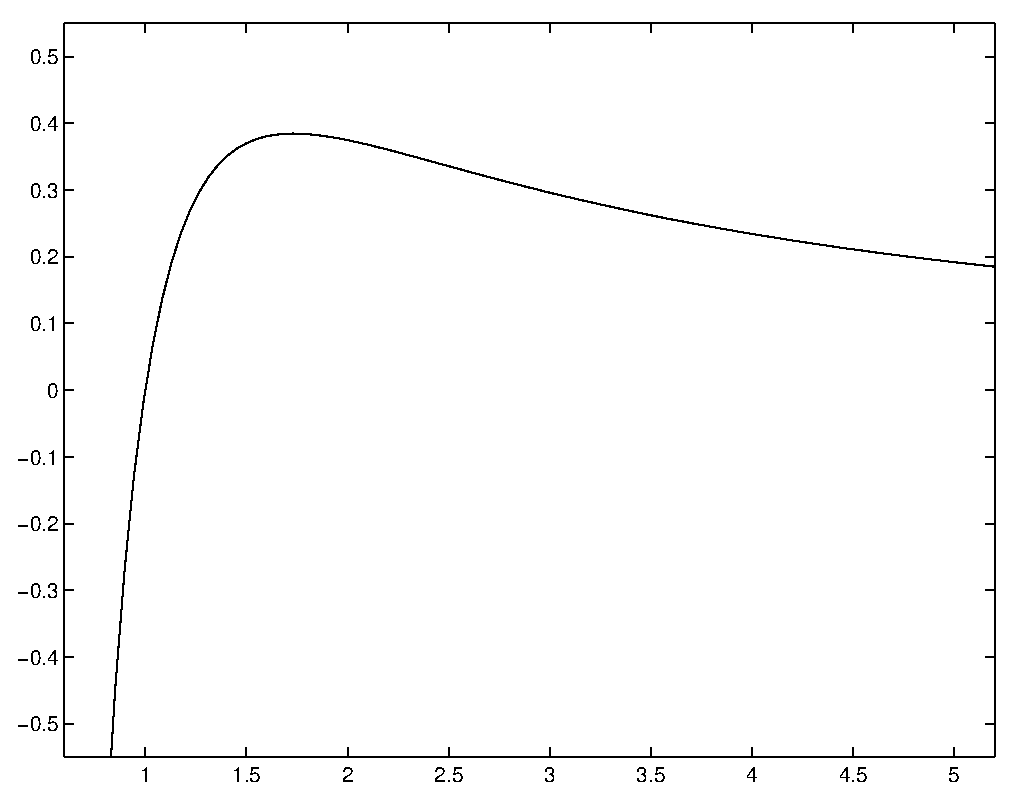
\psfig{file=figures/solnm.eps,width=2.8in}
           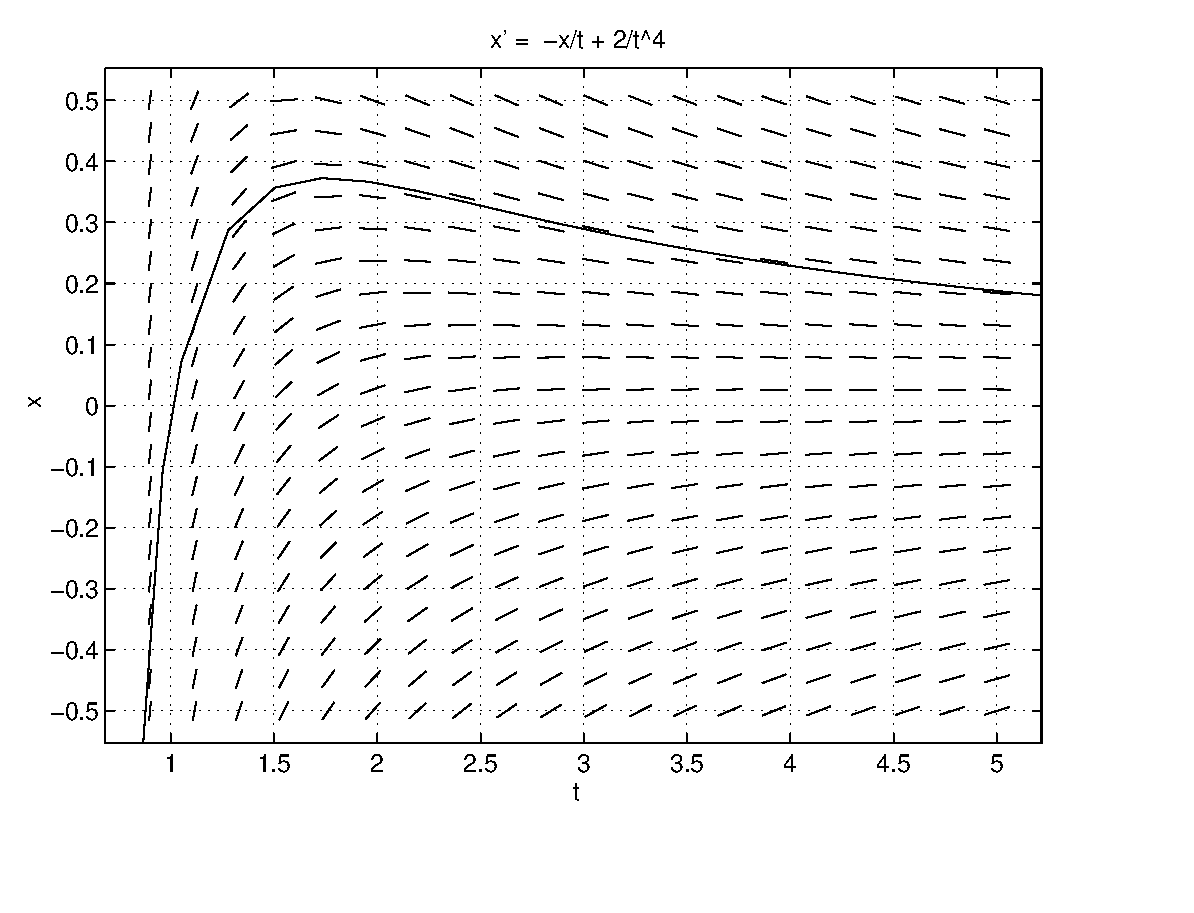
\psfig{file=figures/solnd.eps,width=3.0in}}
           \caption{(Left) Graph of solution~\protect\Ref{e:solnth} to equation 
	\protect\Ref{e:solntheq}. (Right) The time series for solution to 
	\protect\Ref{e:solntheq} with initial condition $x(1)=0$ using 
	{\sf dfield5}.}
           \label{F:solnmd}
\end{figure}

\noindent (b) Solve the initial value problem
\[
\begin{array}{rcl}
\dps \frac{dx}{dt} & = & 4x + \cos t + e^{2t} \\
x(0) & = & 1.
\end{array}
\]
Here $H(t)=4t$ and 
\begin{eqnarray*}
c(t) & = &  \int_0^t g(\tau)e^{-4\tau} d\tau +1\\
& = & \int_0^t \left(\cos\tau + e^{2\tau}\right)e^{-4\tau} d\tau
+1\\
& = & \frac{1}{17}\left( e^{-4t}(\sin t - 4\cos t)+4\right) +
\frac{1}{2}\left(1-e^{-2t}\right) + 1.
\end{eqnarray*}
Thus, the solution is
\[
x(t)=c(t) e^{4t} = \frac{1}{17}(\sin t - 4\cos t+4e^{4t}) -
\frac{1}{2}e^{2t} + \frac{3}{2}e^{4t}.
\]


\EXER

\TEXER 

\noindent In Exercises~\ref{c14.2.1a} -- \ref{c14.2.1f} decide whether 
or not the given differential equation is linear.  If it is linear, 
specify whether the equation is homogeneous or inhomogeneous.
\begin{exercise}  \label{c14.2.1a}
$\dps \frac{dx}{dt} = 0$.
\end{exercise}
\begin{exercise}  \label{c14.2.1b}
$\dps \frac{dx}{dt} = x^2\cos t$.
\end{exercise}
\begin{exercise}  \label{c14.2.1c}
$\dps \frac{dx}{dt} = x+t^2$.
\end{exercise}
\begin{exercise}  \label{c14.2.1d}
$\dps \frac{dx}{dt} = \frac{t}{x}-\frac{1}{t}$.
\end{exercise}
\begin{exercise}  \label{c14.2.1e}
$\dps (t^2+1)\frac{dx}{dt} = x+\sin t$.
\end{exercise}
\begin{exercise} \label{c14.2.1f}
$\dps x\frac{dx}{dt} = \cos t$
\end{exercise}

\noindent In Exercises~\ref{c14.2.6a} -- \ref{c14.2.6d} solve the given 
initial value problems by variation of parameters.
\begin{exercise}   \label{c14.2.6a}
$\dps \frac{dx}{dt} = t^2 x + t^2, \quad x(1)=1$.
\end{exercise}
\begin{exercise}   \label{c14.2.6b}
$\dps \frac{dx}{dt} = x+2t, \quad x(0)=-1$.
\end{exercise}
\begin{exercise}   \label{c14.2.6c}
$\dps \frac{dx}{dt} = 
\frac{t}{t^2+1}x+\sin(t)\sqrt{t^2+1},\quad x(0)=2$.
\end{exercise}
\begin{exercise}   \label{c14.2.6d}
$\dps \frac{dx}{dt} = 2x+\frac{1}{t}e^{2t}, \quad x(1)=4$.
\end{exercise}



\CEXER

\noindent In Exercises~\ref{c14.2.11a} -- \ref{c14.2.11c} use 
{\sf dfield5}\index{\computer!dfield5} 
to compute solutions to the given linear differential equations.  What is 
the asymptotic behavior of the solutions as $t$ tends to infinity?  Use 
variation of parameters to explain the behavior.
\begin{exercise}   \label{c14.2.11a}
$\dps\frac{dx}{dt} = -2 x + t$.
\end{exercise}
\begin{exercise}   \label{c14.2.11b}
$\dps\frac{dx}{dt} = -2 x + t^2$.
\end{exercise}
\begin{exercise}   \label{c14.2.11c}
$\dps\frac{dx}{dt} = -2 x + \sin t$.
\end{exercise}




\Section{Variation of Parameters for Systems}
\label{sec:LinInhomSys}
\index{variation of parameters}

In this section we consider solving inhomogeneous systems of linear
differential equations  of the form
\arraystart
\begin{equation}  \label{eq:linihsys}
\frac{dX}{dt}  =  A(t)X + G(t) 
\end{equation}
\arrayfinish
where $A(t)=(a_{ij}(t))$ is an $n\times n$ matrix and
$G(t)=(g_1(t),\ldots,g_n(t))^t$ is a vector of continuous functions.  
The system is {\em homogeneous\/} when $G(t)=0$.

We divide this discussion into two parts: finding the 
general solution\index{variation of parameters!general solution} 
of the homogeneous\index{homogeneous} equation and finding 
a particular 
solution\index{variation of parameters!particular solution} to the 
inhomogeneous equation using variation of parameters.

\subsection*{Homogeneous Nonconstant Coefficient Systems}

From the theory of constant coefficient systems of linear differential 
equations, we know abstractly how to write  a  basis of solutions to
the homogeneous system  $\dot{X}=AX$ where $A$ is an $n\times n$
constant matrix.  That basis is 
\[
X_j(t) = e^{tA}v_j,
\]
where $\{v_1,\ldots,v_n\}$ is a basis of $\R^n$.  For the 
homogeneous\index{homogeneous} 
system of $n$ nonconstant coefficient linear differential equations
\begin{equation}  \label{E:NCCH}
\dot{X} = A(t) X
\end{equation}
a similar statement is true.   It should be noted, however, that only in 
special cases can \Ref{E:NCCH} be solved in closed form.

\begin{prop}  \label{P:NCCH}
Let $v_1,\ldots,v_n$ be a basis\index{basis} 
for $\R^n$.  Then there exist solutions 
\[
X_1(t),\ldots,X_n(t)
\]
of \Ref{E:NCCH} satisfying $X_j(0)=v_j$ and these
solutions form a basis of solutions\index{basis!of solutions} 
to \Ref{E:NCCH}.
\end{prop}

\proof The theory of differential equations implies that there exists a 
unique solution to \Ref{E:NCCH}  satisfying the initial condition $X(0)=X_0$ 
for any $X_0\in\R^n$.   Therefore, there exist solutions $X_j(t)$ such that 
$X_1(0)=v_j$.  We claim that these solutions form a basis for the vector 
space of all solutions to \Ref{E:NCCH}.   

Let $X(t)$ be any solution to \Ref{E:NCCH} with initial condition $X(0)=X_0$. 
Since $\{X_1(0),\ldots,X_n(0)\}$ is a basis for $\R^n$, we can find scalars 
$\alpha_j$ such that 
\[
X_0 = \alpha_1X_1(0) + \cdots + \alpha_nX_n(0).
\]
Linearity of \Ref{E:NCCH} implies that 
\[
\alpha_1X_1(t) + \cdots + \alpha_nX_n(t)
\]
is a solution.  Therefore, uniqueness of solutions to \Ref{E:NCCH} implies 
that 
\[
X(t) = \alpha_1X_1(t) + \cdots + \alpha_nX_n(t)
\]
for all time $t$, which proves the proposition. \qed

Existence of solutions to the initial value problem $X(t_0)=X_0$ also
guarantees that the vectors $X_1(t_0),\ldots,X_n(t_0)$ must be linearly 
independent\index{linearly!independent}.  
Indeed, since $X_1(t),\ldots,X_n(t)$ is a 
basis of solutions\index{basis!of solutions} to
\Ref{E:NCCH}, we must be able to write 
\[
X_0 = \alpha_1X_1(t_0) + \cdots + \alpha_nX_n(t_0)
\]
for scalars $\alpha_1,\ldots,\alpha_n$ in order for a solution to this 
initial value problem to exist.  That is, the vectors 
$X_1(t_0),\ldots,X_n(t_0)$  must span $\R^n$.   Hence they are linearly 
independent.  We have proved the following:

\begin{lemma}  \label{L:DEspan}
Let $X_1,\ldots,X_n$ be a linearly independent\index{linearly!independent} 
set of solutions to \Ref{E:NCCH}.
Then, for every $t$, the matrix 
\begin{equation}   \label{E:Y(t)}
Y(t) = \left(X_1(t)|\cdots |X_n(t)\right) 
\end{equation}
is invertible\index{invertible}.
\end{lemma}

\proof  Proposition~\ref{P:NCCH} implies that the columns of $Y(t)$ are 
linearly independent.  Hence $Y(t)$ is invertible.  \qed

Rather than relying on the general existence and uniqueness theory for
systems of differential equations, there is a computationally direct way of 
proving Lemma~\ref{L:DEspan}.   It is possible to show that the determinant 
of the matrix $Y(t)$ in \Ref{E:Y(t)} is nonzero and hence $Y(t)$ is invertible.
This approach is carried out in Section~\ref{S:wronskian}


\subsection*{The Theory of Variation of Parameters}
\index{variation of parameters!theory}

Let $X_1(t),\ldots,X_n(t)$ be a 
basis of solutions\index{basis!of solutions} to the homogeneous 
system $\dot{X}=A(t)X$.   In the method of variation of parameters we look 
for solutions to  the inhomogeneous system \Ref{eq:linihsys} of the form
\[
X(t) = c_1(t)X_1(t) + \cdots + c_n(t)X_n(t),
\]
where $c_1(t),\ldots,c_n(t)$ are differentiable functions.  In order to 
find a method for determining the functions $c_j$, we assume that $X$ is 
a solution to \Ref{eq:linihsys}.  

Use the product rule\index{product rule} to compute
\begin{eqnarray*}
\dps\frac{dX}{dt} & = &\sum_{j=1}^n\left(c_j\frac{dX_j}{dt}
+\frac{dc_j}{dt} X_j\right)\\
& = & \sum_{j=1}^n\left( c_jAX_j+\frac{dc_j}{dt}X_j\right)\\
& = & AX+\sum_{j=1}^n \frac{dc_j}{dt}X_j.
\end{eqnarray*}
It follows that $X$ is a solution of \Ref{eq:linihsys} if and only if
\begin{equation}  \label{eq:dcjXj}
G(t) = \frac{dc_1}{dt}(t) X_1(t) + \cdots + \frac{dc_n}{dt}(t) X_n(t).
\end{equation}
So variation of parameters works if we can find functions $c_j$ that 
satisfy \Ref{eq:dcjXj}.

We claim that it is always possible to find functions $d_j(t)$ so that 
\begin{equation}  \label{E:djXj}
G(t) = d_1(t)X_1(t) + \cdots + d_n(t)X_n(t).
\end{equation} 
To verify \Ref{E:djXj}, note that  \Ref{E:djXj} can be rewritten in matrix 
form as
\[
Y(t) D(t) = G(t)
\]
where $Y(t)$ is defined in \Ref{E:Y(t)} and
\[
D(t)=(d_1(t),\ldots,d_n(t))^t.
\]
Using the invertibility\index{invertible} of 
$Y(t)$, as proved in Lemma~\ref{L:DEspan}, we find that
\[
D(t) = Y(t)\inv G(t).
\] 
It now follows that \Ref{eq:dcjXj} is satisfied by integrating the 
differential equations $\dot{c}_j=d_j$, where the functions $d_j(t)$ 
are defined in \Ref{E:djXj}, to find the functions $c_j$.  

We summarize this discussion as follows. 
\begin{thm}[Variation of Parameters: Systems] \label{thm:varparsys}
\index{variation of parameters!for systems}
Consider 
\begin{equation}  \label{eq:VPS}
\begin{array}{rcl}
\dps \frac{dX}{dt} & = & A(t)X+G(t)\\
X(t_0) & = & X_0.
\end{array}
\end{equation}
\begin{itemize}
\item[(a)]  Let $X_1(t),\ldots,X_n(t)$ be a 
basis of solutions\index{basis!of solutions} to 
the homogeneous differential equation $\dot{X}=A(t)X$.  
\item[(b)]  Let $Y(t)$ be defined as in \Ref{E:Y(t)} and define 
$D(t)=(d_1(t),\ldots,d_n(t))^t$ by 
\begin{equation}  \label{e:D(t)}
D(t) = Y(t)\inv G(t).
\end{equation}
\item[(c)]  Let the functions $c_1(t),\ldots,c_n(t)$ satisfy the initial 
value problem\index{variation of parameters!initial value problem} 
\begin{equation}  \label{eq:cj0}
\frac{dc_j}{dt}=d_j \AND  c_1(t_0)X_1(t_0) + \cdots +c_n(t_0)X_n(t_0) = X_0.
\end{equation}
\end{itemize}
Then
\[
X(t) =  c_1(t)X_1(t) + \cdots + c_n(t)X_n(t)
\]
is the unique solution\index{uniqueness of solutions} of \Ref{eq:VPS}.
\end{thm}

Note that when $n\ge 3$, the hand computation of $Y(t)\inv$ can be  
painful.

\subsection*{Examples with Constant Coefficient Matrix $A$ when $n=2$}

We consider two examples of variation of parameters applied to 
forced systems of differential equations of the form 
\[
\dot{X} = AX + G(t).
\]

\subsubsection*{An Example with Two Real Simple Eigenvalues}

Consider the initial value problem \Ref{eq:VPS} where
\begin{equation}  \label{eq:exinhom2}
A=\mattwo{-1}{-8}{-16}{7}, \quad G(t)= \vectwo{1-t}{-2-t}, \quad 
X_0 =  \vectwo{-1}{-1}.
\end{equation}
Variation of parameters proceeds in four steps:

\paragraph{Step 1: Solutions to the homogeneous equation.} The 
eigenvalues\index{eigenvalue!real!distinct} and 
eigenvectors\index{eigenvector} of $A$ can be 
found either by using \Matlab or by hand.  The eigenvalues are $\lambda_1=-9$ 
and $\lambda_2=15$, and the associated eigenvectors are $v_1=(1,1)^t$ 
and $v_2=(1,-2)^t$.  Therefore, solutions of the homogeneous equation are:
\[
X_1(t) = e^{-9t}\vectwo{1}{1} \AND X_2(t) = e^{15t}\vectwo{1}{-2}.
\]

\paragraph{Step 2: Computation of the vector $D(t)$.}   We compute the inverse 
\[
Y(t)\inv = \mattwo{e^{-9t}}{e^{15t}}{e^{-9t}}{-2e^{15t}}\inv = 
-\frac{1}{3e^{6t}}\mattwo{-2e^{15t}}{-e^{15t}}{-e^{-9t}}{e^{-9t}} =
\frac{1}{3}\mattwo{2e^{9t}}{e^{9t}}{e^{-15t}}{-e^{-15t}}.
\]
The vector $D(t)$ is:
\[
D(t) = Y(t)\inv G(t) = 
\frac{1}{3}\mattwo{2e^{9t}}{e^{9t}}{e^{-15t}}{-e^{-15t}}\vectwo{1-t}{-2-t}
= \vectwo{-te^{9t}}{e^{-15t}}
\]

\paragraph{Step 3: Computation of the functions $c_j(t)$.}   By assumption 
\[
X_0=c_1(0)X_1(0)+c_2(0)X_2(0).
\]
Therefore
\[
\vectwo{-1}{-1} = c_1(0)\vectwo{1}{1} + c_2(0)\vectwo{1}{-2},
\]
from which it follows that $c_1(0)=-1$ and $c_2(0)=0$.  Since
\[
\dot{c}_1 = d_1 = -te^{9t}  \AND \dot{c}_2 = d_2 = e^{-15t},
\]
it follows that 
\[
\begin{array}{rclcl}
c_1(t) & = & \int_0^t (-\tau) e^{9\tau}d\tau - 1
& = &  -\frac{1}{9}\left(t-\frac{1}{9}\right)e^{9t}-\frac{82}{81} \\
c_2(t) & = & \int_0^t e^{-15t}d\tau & = & \frac{1}{15}\left(1-e^{-15t}\right).
\end{array}
\]

\paragraph{Step 4: Write out the solution.}  The solution $X(t)$ of the 
initial value problem \Ref{eq:exinhom2} is now given by
\begin{eqnarray*}
X(t) & = & c_1(t)e^{-9t}\vectwo{1}{1} + c_2(t)e^{15t}\vectwo{1}{-2} \\
& = &  \left(\begin{array}{c}
-\frac{1}{9}\left(t-\frac{1}{9}\right)-
\frac{82}{81}e^{-9t}+\frac{1}{15}\left( e^{15t}-1\right)\\
-\frac{1}{9}\left(t-\frac{1}{9}\right)-
\frac{82}{81}e^{-9t}-\frac{2}{15}\left( e^{15t}-1\right)
\end{array}\right).
\end{eqnarray*}

\subsubsection*{An Example with a Nontrivial Jordan Block}
\index{Jordan block}

Solve the system
\begin{equation}  \label{e:2djb}
\begin{array}{rcl}
\dot{X} & = & A X + (t,1)^t \\
X(0) & = & (1,-1)^t,
\end{array}
\end{equation}
where 
\[
A = \mattwo{2}{1}{0}{2}.
\]

\paragraph{Step 1:}  A basis for solutions to the homogeneous equation 
$\dot{X}=AX$ is
\[
X_1(t) = e^{2t}\vectwo{1}{0} \AND X_2(t) = e^{2t}\vectwo{t}{1}.
\]

\paragraph{Step 2:}  We compute
\[
D(t) =  e^{-2t}\mattwo{1}{t}{0}{1}\inv G(t) = 
e^{-2t}\mattwo{1}{-t}{0}{1}\vectwo{t}{1} = e^{-2t}\vectwo{0}{1}.
\]

\paragraph{Step 3:}  Note that 
\[
X(0) = \vectwo{1}{-1} = c_1(0)\vectwo{1}{0} + c_2(0)\vectwo{0}{1}.
\]
So $c_1(0)=1$ and $c_2(0)=-1$.  Now solve the differential equations
\[
\begin{array}{rclcl}
\dot{c}_1 & = & d_1(t) & = & 0 \\
\dot{c}_2 & = & d_2(t) & = & e^{-2t},
\end{array}
\]
obtaining
\begin{eqnarray*}
c_1(t) & = & 1 \\
c_2(t) & = & -\frac{1}{2}(e^{-2t}+1).
\end{eqnarray*}

\paragraph{Step 4:}  It follows from Theorem~\ref{thm:varparsys} that the 
solution to \Ref{e:2djb} is
\[
X(t) = c_1(t)X_1(t) + c_2(t)X_2(t) = -\frac{1}{2}\left(\begin{array}{c}
t(1+e^{2t})-2e^{2t} \\ e^{2t}+1 \end{array}\right).
\]
 


\EXER

\TEXER

\noindent In Exercises~\ref{c14.3.1a} -- \ref{c14.3.1b} solve the given 
initial value problems by variation of parameters.

\begin{exercise}  \label{c14.3.1a}
\[
\frac{dX}{dt}=\frac{1}{2}\mattwo{1}{1}{1}{1} X + \vectwo{e^t}{0},\quad
X(0) = \vectwo{1}{-1}.
\]
\end{exercise}
\begin{exercise}  \label{c14.3.1b}
\[
\frac{dX}{dt}=\mattwo{1}{3}{3}{1} X + \vectwo{2t}{t},\quad
X(0) = \vectwo{0}{1}.
\]
\end{exercise}

\begin{exercise}  \label{c17.3.3}
Find the general solution to the system of differential equations
\[
\frac{dX}{dt}= \mattwo{-\frac{1}{t}}{\frac{1}{t^2}}{1}{0}X+\vectwo{1}{3t}.
\]
{\bf Hint:} Verify that 
\[
X_1(t) = \vectwoc{1}{t} \AND X_2(t) = \vectwo{\frac{1}{t^2}}{-\frac{1}{t}}
\]
are solutions to the homogeneous equation and then use variation of parameters.
\end{exercise}

\begin{exercise}  \label{c17.3.4}
Find the general solution to the system of differential equations
\[
\frac{dX}{dt}= \mattwoc{0}{1}{\frac{3}{t^2}}{\frac{1}{t}}X+\vectwoc{t}{2t}.
\]
{\bf Hint:} Verify that 
\[
X_1(t) = \vectwoc{t^3}{3t^2}\AND X_2(t) = \vectwoc{\frac{1}{t}}{-\frac{1}{t^2}}
\]
are solutions to the homogeneous equation and then use variation of parameters.
\end{exercise}






\Section{The Wronskian}  \label{S:wronskian}
\index{Wronskian} 

We return to the homogeneous system of linear differential equations
\arraystart
\begin{equation}  \label{eq:linihsys2}
\frac{dX}{dt}  =  A(t)X
\end{equation}
\arrayfinish
where $A(t)=(a_{ij}(t))$ is an $n\times n$ matrix.  Let $X_1,\ldots,X_n$ be a 
linearly independent set of solutions\index{basis!of solutions} 
to \Ref{eq:linihsys2} and let 
\begin{equation}   \label{E:Y(t)2}
Y(t) = \left(X_1(t)|\cdots |X_n(t)\right) 
\end{equation}
Using existence and uniqueness of solutions to the initial problem for
\Ref{eq:linihsys2}, we showed in Lemma~\ref{L:DEspan} that $Y(t)$ is an 
invertible matrix for every time $t$.  In this section we prove this same 
result by explicitly showing that the determinant\index{determinant} 
of $Y(t)$ is always nonzero.

Define the {\em Wronskian\/}\index{Wronskian} to be
\[
W(t) = \det Y(t).
\]

\begin{thm}  \label{T:Wronskian}
Let $X_1,\ldots,X_n$ be solutions to \Ref{E:NCCH} such that the vectors
$X_j(0)$ form a basis of $\R^n$.  Let $Y(t)$ be the matrix defined in 
\Ref{E:Y(t)}.  Then
\begin{equation}  \label{L:Wronskian}
W(t) = e^{\int_0^t\trace(A(\tau))d\tau}W(0).
\end{equation}
\end{thm}

It follows directly from \Ref{L:Wronskian} that the determinant of $Y(t)$ is 
nonzero when the determinant of $Y(0)$ is nonzero.  But $\det Y(0)\neq 0$ 
since the vectors $X_j(0)$ form a basis of $\R^n$. 

We prove Theorem~\ref{T:Wronskian} in two important special cases: linear 
constant coefficient systems and linear nonconstant $2\times 2$ systems.  
The proof for constant coefficient systems is based on Jordan normal forms, 
while the proof for $2\times 2$ systems is based on solving a separable 
differential equation for the Wronskian itself.  It is this latter proof 
that generalizes to a proof of the theorem.

\subsubsection*{Wronskians for Constant Coefficient Systems}
\index{Wronskian!constant coefficient system}

First, we interpret the Wronskian directly in terms of the constant coefficient 
matrix $A$.  Note that $X_j(t)=e^{tA}e_j$ is just the $j^{th}$ column of the 
matrix $e^{tA}$.   It follows that 
\[
W(t) = \det e^{tA}.
\]

\begin{lemma} 
Let $A$ be an $n\times n$ matrix.  Then
\[
\det e^A = e^{\trace(A)}.
\]
\end{lemma}\index{determinant}\index{matrix!exponential}
\index{trace}

\proof  This result is proved using 
Jordan normal forms\index{Jordan normal form}.  To see why normal
form theory is relevant, suppose that $A$ and $B$ are similar matrices.  Then 
$e^A$ and $e^B$ are similar matrices, and $\trace(A)=\trace(B)$ and 
$\det e^A = \det e^B$.  So if we can show that the lemma is valid for matrices 
in Jordan normal form, then the lemma is valid for all matrices.

Suppose that the matrix $J$ is  a $k\times k$ 
Jordan block\index{Jordan block} matrix associated
to the eigenvalue $\lambda$.  Then $J$ is upper triangular and the 
diagonal entries of $J$ all equal $\lambda$.  
It follows that $\trace(J)=k\lambda$.
It also follows that $e^J$ is an upper triangular matrix whose diagonal 
entries all equal $e^\lambda$.  Hence
\[
\det e^J = \left(e^\lambda\right)^k = e^{k\lambda} = e^{\trace(J)}.
\]
So the lemma is valid for Jordan block matrices.

Next suppose that $A$ is in block diagonal\index{matrix!block diagonal}, 
that is
\[
A=\mattwo{B}{0}{0}{C}.
\]
We claim that if the lemma is valid for matrices $B$ and $C$, then it 
is valid for the matrix $A$.  To see this observe that 
\[
\trace(A) = \trace(B) + \trace(C),
\]
and that 
\[
e^A = \mattwo{e^B}{0}{0}{e^C}.
\]
Hence 
\[
\det e^A = \det e^B \det e^C = e^{\trace(B)}e^{\trace(C)}, 
\]
by assumption.  It follows that 
\[
\det e^A = e^{\trace(B)+\trace(C)} = e^{\trace(A)},
\]
as desired.  By induction,  the lemma is valid for Jordan normal form 
matrices and hence for all matrices.  \qed

\subsubsection*{Wronskians for Planar Systems}
\index{Wronskian!planar system}

In the time dependent case we verify Theorem~\ref{T:Wronskian} only 
for $2\times 2$ systems, as this 
substantially simplifies the discussion.   Let 
\[
A(t) = \mattwo{a_{11}(t)}{a_{12}(t)}{a_{21}(t)}{a_{22}(t)},
\]
and let 
\[
X_1(t) = \vectwo{x_1(t)}{y_1(t)} \AND  X_2(t) = \vectwo{x_2(t)}{y_2(t)}
\]
be solutions of \Ref{E:NCCH}.  It follows that 
\begin{equation}   \label{E:xyderiv}
\begin{array}{rcl}
\dot{x}_1 & = & a_{11}x_1 + a_{12}y_1 \\
\dot{y}_1 & = & a_{21}x_1 + a_{22}y_1 \\
\dot{x}_2 & = & a_{11}x_2 + a_{12}y_2 \\
\dot{y}_2 & = & a_{21}x_2 + a_{22}y_2.
\end{array}
\end{equation}

In this notation 
\[
Y(t) = \mattwo{x_1(t)}{x_2(t)}{y_1(t)}{y_2(t)},
\]
and
\[
W(t) = x_1(t)y_2(t) - x_2(t)y_1(t).
\]
We claim that 
\[
\dot{W} = \trace(A) W.
\]
If so, we can use separation of variables to solve this differential equation 
obtaining
\[
\ln |W| = \int \trace(A(t))dt 
\]
from which the proof of Theorem~\ref{T:Wronskian} follows.

Use the product rule to compute
\[
\dot{W}  =  \dot{x}_1y_2 + x_1\dot{y}_2 - \dot{x}_2y_1 - x_2\dot{y}_1.
\]
Now substitute \Ref{E:xyderiv} to see that 
\[
\dot{W} = (a_{11}x_1 + a_{12}y_1)y_2 + x_1(a_{21}x_2 + a_{22}y_2)
- (a_{11}x_2 + a_{12}y_2)y_1 - x_2(a_{21}x_1 + a_{22}y_1)
\]
from which it follows that 
\[
\dot{W} = (a_{11}+a_{22})W = \trace(A)W,
\]
as claimed.
\qed


\EXER

\TEXER

In Exercises~\ref{c14.4.1a} -- \ref{c14.4.1d} compute the Wronskian
$W(t)$ for the specified matrices:

\begin{exercise} \label{c14.4.1a}
$Y(t) = \mattwo{t}{1}{-1}{t}$.
\end{exercise}

\begin{exercise} \label{c14.4.1b}
$Y(t) = \mattwo{\cos t}{-\sin t}{\sin t}{\cos t}$.
\end{exercise}

\begin{exercise} \label{c14.4.1c}
$Y(t) = \left(\begin{array}{ccc}
0 & t & e^t\\  1 & t & te^t \\ t & t & t^2 e^t \end{array}\right)$.
\end{exercise}

\begin{exercise} \label{c14.4.1d}
$Y(t) = \left(\begin{array}{ccc}
1 & 0 & 1\\  1 + \sin t & 1 & e^t \\ -4 + \cos t & t & te^t 
\end{array}\right)$.
\end{exercise}

\begin{exercise}  \label{c14.w.2}
Use \Ref{L:Wronskian} to verify that the Wronskian for solutions to the linear 
constant coefficient system of ODE $\dot{X}=AX$ is
\begin{equation}  \label{E:ccw}
W(t) = e^{\trace(A)t}W(0).
\end{equation}
\end{exercise}

\noindent In Exercises~\ref{c14.w.3a} -- \ref{c14.w.3c} verify \Ref{E:ccw} 
for the given matrix $A$.  {\bf Hint:} First, you need to find linearly 
independent solutions to the system $\dot{X}=AX$.
\begin{exercise} 	\label{c14.w.3a}
$A = \mattwo{0}{-1}{1}{0}$.
\end{exercise}
\begin{exercise} 	\label{c14.w.3b}
$A = \mattwo{2}{3}{3}{2}$.
\end{exercise}
\begin{exercise} 	\label{c14.w.3c}
$A = \mattwo{2}{-2}{4}{-3}$.
\end{exercise}

 


\Section{Higher Order Equations}
\label{S:RO}

Using the same trick as in the case of equations with constant 
coefficients we can rewrite a higher order linear equation with
nonconstant coefficients as a first order system of linear
equations.  This way we can also use the method of variation 
of parameters for the solution of higher order equations.  
In fact, consider a general linear differential equation of 
order\index{order} $n$
\begin{equation}
\label{E:noncc}
\frac{d^nx}{dt^n} + a_{n-1}(t)\frac{d^{n-1}x}{dt^{n-1}} +\cdots + 
a_1(t)\frac{dx}{dt}+a_0(t)x = g(t).
\end{equation}\index{differential equation!higher order}
As in Section~\ref{sec:HighOrder} we define the functions
$x_1(t),\ldots,x_n(t)$ by
\[
x_1(t)=x(t),\quad x_2(t)=\frac{dx}{dt}(t),\quad
\ldots, \quad  x_n(t)=\frac{d^{n-1}x}{dt^{n-1}}(t)
\]
and see that \Ref{E:noncc} is equivalent to
\arraystart
\[
\begin{array}{rcl}
\dps \frac{dx_j}{dt}&=&x_{j+1} \hspace{1.6in} (j=1,\ldots,n-1)\\
\dps \frac{dx_n}{dt}&=& g(t) - a_0(t)x_1 - \cdots - a_{n-1}(t) x_n.
\end{array}
\]
\arrayfinish
Introducing the vectors
\[
X(t) = (x_1(t),\ldots,x_n(t))^t  \AND
G(t) = (0,\ldots,0,g(t))^t
\]
we conclude that \Ref{E:noncc} is equivalent to the 
first order system\index{first order!reduction to}
\[
\frac{dX}{dt} = A(t)X+G(t),
\]
where $A(t)$ is the matrix
\[
A(t) = \left(\begin{array}{ccccc}
0 & 1 & 0 & \cdots & 0\\
0 & 0 & 1 & \cdots & 0\\
\vdots & \vdots & \vdots & & \vdots\\
0 & 0 & 0 & \cdots & 1\\
-a_0(t) & -a_1(t) &  -a_2(t) & \cdots & -a_{n-1}(t)
\end{array}\right).
\]
In particular, $x_1(t)$ is a solution of \Ref{E:noncc} if 
$X(t)=(x_1(t),\ldots,x_n(t))^t$ is a solution of the system
$\dot X = A(t)X+G(t)$ which can in principle be solved by
variation of parameters.

\subsubsection*{An Example of Second Order}

As an example we find a solution to the initial value
problem 
\begin{equation}
\label{E:2ndorderex}
\begin{array}{c}
\dps \ddot x - \frac{2}{t} \dot x + \frac{2}{t^2} x = t,\\
\dps x(1) = 0,\quad \dot x(1) = 1.
\end{array}
\end{equation}
This second order differential equation is equivalent to the system
\begin{equation}  \label{E:2ndexam}
\begin{array}{rcl}
\dps \dot{X} & = & A(t) X + G(t) \\
\dps X(1) & = & (0,1)^t,
\end{array}
\end{equation}
where 
\[
A(t) = \mattwo{0}{1}{-\frac{2}{t^2}}{\frac{2}{t}}\AND G(t) = \vectwo{0}{t}.
\]

\paragraph{Step 1:}  A basis of solutions\index{basis!of solutions} 
to the homogeneous equation $\dot X = A(t)X$ is
\[
X_1(t) = \vectwo{t}{1} \AND X_2(t) = \vectwo{t^2}{2t}.
\]

\paragraph{Step 2:}  The inverse of $Y(t)$ is given by
\[
Y(t)^{-1} = \frac{1}{t^2} \mattwo{2t}{-t^2}{-1}{t}.
\]
Hence we obtain
\[
D(t) = Y(t)^{-1} G(t) = \frac{1}{t^2} \mattwo{2t}{-t^2}{-1}{t}\vectwo{0}{t}  
= \vectwo{-t}{1}
\]

\paragraph{Step 3:} Note that 
\[
X(1) = \vectwo{0}{1} = c_1(1)\vectwo{1}{1} + c_2(1)\vectwo{1}{2}.
\]
So $c_1(1)=-1$ and $c_2(1)=1$.  Now solve the differential equations
\[
\begin{array}{rclcl}
\dot{c}_1 & = & d_1(t) & = & -t \\
\dot{c}_2 & = & d_2(t) & = & 1,
\end{array}
\]
with these initial conditions obtaining
\begin{eqnarray*}
c_1(t) & = & -\frac{1}{2}(t^2+1) \\
c_2(t) & = & t.
\end{eqnarray*}

\paragraph{Step 4:}  Theorem~\ref{thm:varparsys} implies that the 
solution to \Ref{E:2ndexam} is
\[
X(t) = c_1(t)X_1(t) + c_2(t)X_2(t) = \left(\begin{array}{c}
\frac{t}{2}(t^2-1)\\ \frac{1}{2}(3t^2-1) \end{array}\right),
\]
and hence the solution of \Ref{E:2ndorderex} is given by
\[
x(t) = \frac{t}{2}(t^2-1).
\]

\subsubsection*{An Example of an Electrical Circuit}
\index{RLC circuit}\index{electrical circuit}

It is rare, however, that variation of parameters can actually be 
used to find a closed form solution\index{closed form solution} 
to an inhomogeneous higher order 
linear differential equations with variable coefficients.  In such 
instances it is best to resort to numerical integration of the first 
order system obtained from the higher order equation.   

We consider here the temporal behavior of an RLC-circuit introduced in 
Section~\ref{S:SOFE}.  This circuit is described by the differential equation
\[
\ddot x + \frac{R}{L}\dot x +
\frac{1}{CL}x = \frac{1}{CL}V(t),
\]
where $x(t)$ is the voltage drop at the capacitor,
\index{capacitor}\index{resistor}\index{coil}
$R$ is the resistance, $L$ is the inductance,
$C$ is the capacitance, and a voltage source\index{voltage source} 
is producing a time 
dependent voltage $V(t)$, see \Ref{e:eleccirc} in Chapter~\ref{C:LT}.
Now we assume that the circuit additionally
contains a microphone\index{microphone} that has a time dependent 
resistance $R_{mic}(t)$ of the form
\[
R_{mic}(t) = R_0 + R_1\cos(\omega t).
\]
This corresponds to the fact that a periodic signal of 
frequency\index{frequency} 
$\frac{2\pi}{\omega}$ is entering the microphone.  Then
the differential equation for the electrical circuit becomes
\begin{equation}
\label{E:RCLMcir}
\ddot x + \frac{R+R_{mic}(t)}{L}\dot x +
\frac{1}{CL}x = \frac{1}{CL}V(t).
\end{equation}
For simplicity we set
\[
R=0 \AND C=L=R_0 = R_1 = \omega = 1
\]
and assume that the voltage source is producing the constant voltage
\[
V(t) = 1.
\]
Thus we obtain the following linear differential equation of second order
\[
\ddot x + (1+\cos t)\dot x + x = 1,
\]
which is equivalent to the system $\dot X= A(t)X + G(t)$, where
\begin{equation*} \label{E:RCLM}
A(t) = \left( \begin{array}{cc}0 & 1\\-1 & -(1+\cos t)\end{array}\right)
\AND G(t) = \vectwo{0}{1}.
\end{equation*}
It is not obvious how to find the general solution\index{general solution} 
of this equation by hand.
In fact, it is not even clear how to construct solutions of the
homogeneous equation.  Hence we have to rely on numerical methods
and compute solutions using {\tt ode45}\index{\computer!ode45} 
in \Matlabp.  The right hand
side in \Ref{E:RCLM} is stored in the function m-file {\tt f17\_4\_5.m}.
For completeness,
\begin{verbatim}
function f = f17_4_5(t,x)
A = [0  1; -1  -(1+cos(t))];
f = A*x + [0; 1];
\end{verbatim}
We compute the solution of \Ref{E:RCLM} with initial condition $X(0)=(1,1)^t$
for $t\in[0,30]$ by typing
\begin{verbatim}
[t,x] = ode45('f17_4_5',[0 30],[1,1]');
\end{verbatim}
The result of this computation is shown in Figure~\ref{Fig:micro1}.
\begin{figure}[htb]
 \centerline{%
           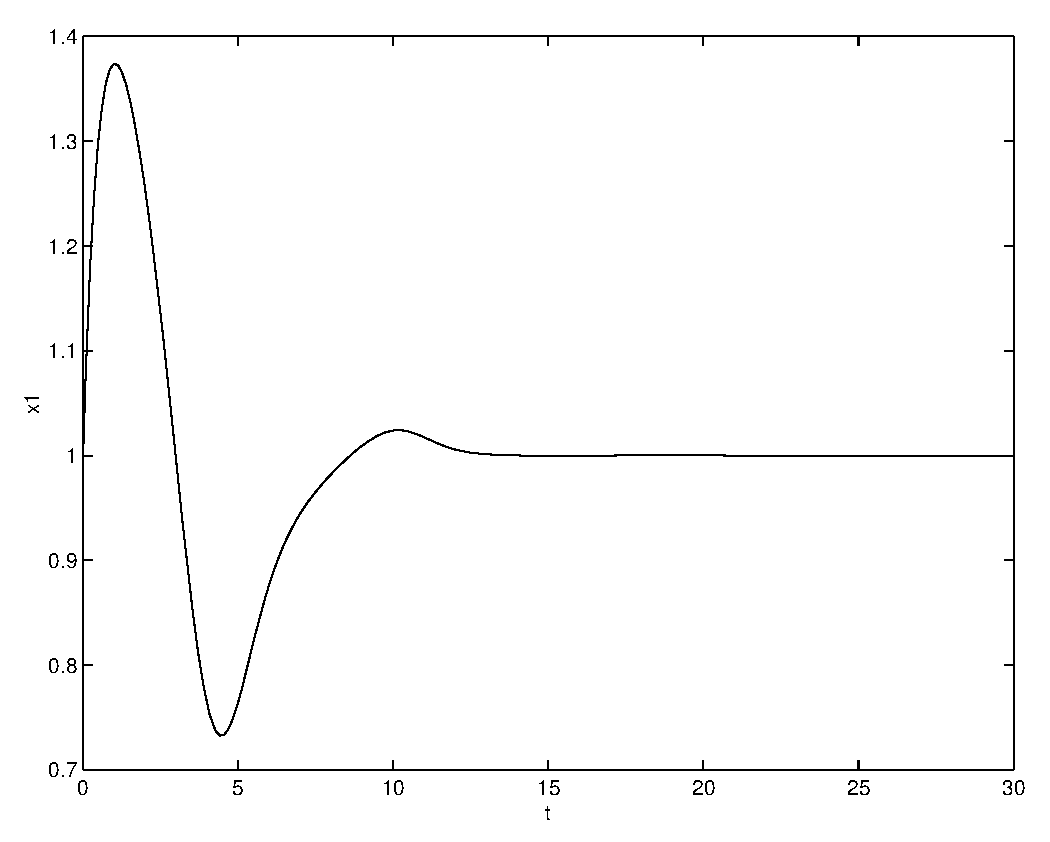
\psfig{file=figures/microx1.eps,width=3.0in}
	   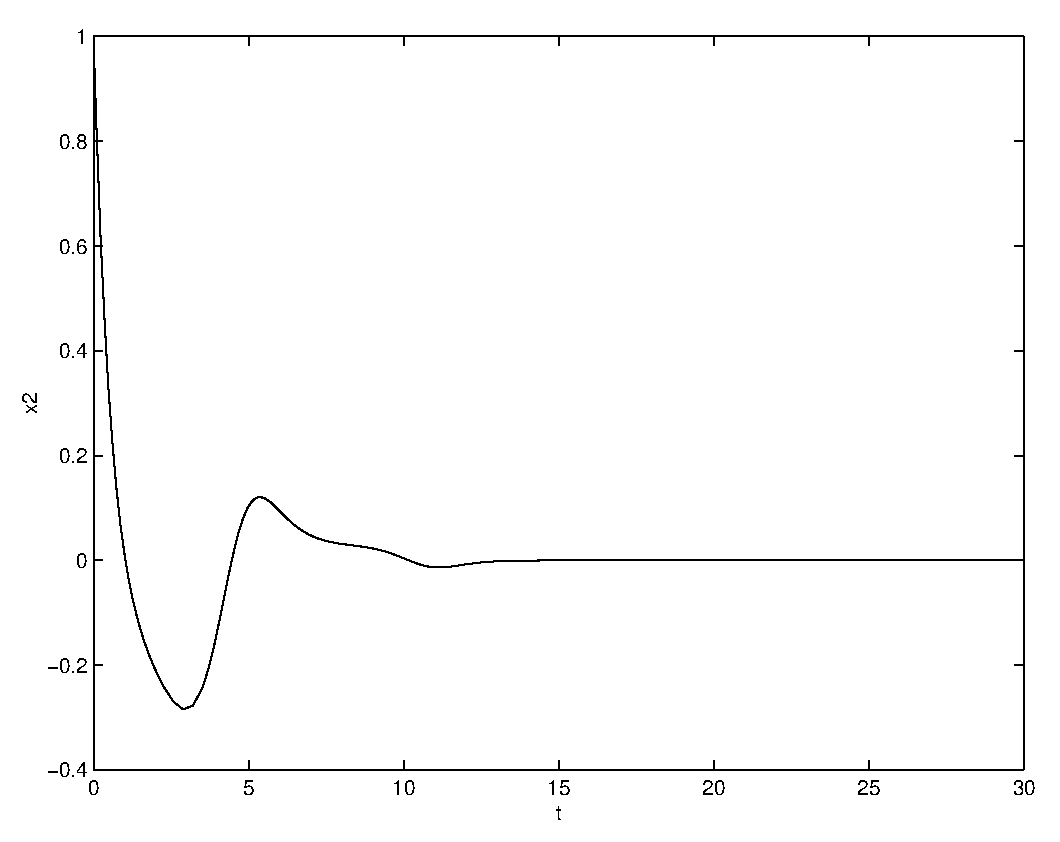
\psfig{file=figures/microx2.eps,width=3.0in}}
           \caption{The two components of the solution of 
	   \protect\Ref{E:RCLM} for $t\in[0,30]$ with initial
	   condition $X(0)=(1,1)^t$.}
           \label{Fig:micro1}
\end{figure}
It can be observed that $x_1(t)$ tends to $1$ and $x_2(t)$ tends to
$0$ for increasing time $t$.  In other words, the solution approaches the 
time independent solution $X(t)=(1,0)^t$ of \Ref{E:RCLM}.

\subsection*{Reduction of Order}
\index{reduction of order}

In order to find solutions to a higher order linear differential equation 
we have rewritten the higher order equation as a first order
system of linear equations, and then we applied variation of
parameters to that system.  There is another method known as
{\em reduction of order\/} that uses the same idea for the
construction principle of the solution --- but this idea is applied directly 
to the higher order equation.  We remark that {\em reduction of
order\/} can sometimes work even when a method like undetermined 
coefficients fails, since its applicability does not depend on the 
specific type of the inhomogeneity.  However, as in the case 
of variation of parameters, the practical use of this technique is very 
limited.  The reason is that the integrations that are involved in the 
computations can rarely be performed by hand.


We illustrate this method by the second order linear differential 
equation
\begin{equation}  \label{e:inhom2}
\ddot{x} + a_1(t)\dot{x} + a_0(t)x = g(t).
\end{equation}
Roughly speaking, reduction of order is a way to reduce the second order 
inhomogeneous equation to an inhomogeneous first order equation.

Suppose that $x_h(t)$ is a solution of the 
homogeneous\index{homogeneous} second order equation
$\ddot{x} + a_1(t)\dot{x} + a_0(t)x = 0$.  
In analogy to the method of variation of
parameters, we try to find a solution $x(t)$ of the 
inhomogeneous\index{inhomogeneous} equation
\Ref{e:inhom2} of the form
\[
x(t) = c(t) x_h(t),
\]
where $c(t)$ is a smooth function.  To determine $c(t)$ we substitute $x(t)$
into the inhomogeneous equation \Ref{e:inhom2}.  Before proceeding, we
compute the derivatives of $x(t)$:
\begin{eqnarray*}
\dot x  & = & \dot c x_h + c \dot{x}_h,\\
\ddot x & = & \ddot c x_h + 2 \dot c \dot{x}_h + c \ddot{x}_h.
\end{eqnarray*}
Next, we substitute $\dot{x}$ and $\ddot{x}$ into \Ref{e:inhom2} and find
\begin{eqnarray*}
&& \ddot c x_h +2\dot c \dot{x}_h + c \ddot{x}_h +
a_1(t)\left(\dot c x_h + c \dot{x}_h \right)+ a_0(t) c x_h =\\
&& x_h \left(\ddot c + \dot c(2 \frac{\dot{x}_h}{x_h} + a_1(t))\right) +
 c(\ddot{x}_h +a_1(t) \dot{x}_h +a_0(t) x_h) = g(t).
\end{eqnarray*}
Since $x_h$ is a solution of the homogeneous equation we have that
$\ddot{x}_h +a_1(t) \dot{x}_h +a_0(t)x_h=0$. After dividing by $x_h$ the function
$c(t)$ satisfies
\[
\ddot c + \dot c\left( 2\frac{\dot{x}_h}{x_h} +a_1(t)\right) = \frac{g(t)}{x_h}.
\]
Introducing $y(t)=\dot c(t)$, we arrive at the differential equation
\[
\frac{dy}{dt} = -y\left( 2\frac{\dot{x}_h}{x_h} +a_1(t)\right) + \frac{g(t)}{x_h}
\]
which is linear and of first order.  If we can find a solution
$y(t)$ of this equation then we can compute $c(t)$ by integration
and we have constructed a 
particular solution\index{reduction of order!particular solution} 
$x(t)=c(t)x_h(t)$ of the
inhomogeneous equation \Ref{e:inhom2}. Thus
\begin{thm}[Reduction of Order]  \label{thm:redord}
Consider the inhomogeneous linear ODE of second order \Ref{e:inhom2}.
\begin{itemize}
\item[(a)] Let $x_h(t)$ be a nonzero solution of the homogeneous equation
\[
\ddot{x} + a_1(t)\dot{x} + a_0(t)x = 0.
\]
\item[(b)] Let $c(t)$ be a function such that its derivative 
$\dot c(t)$ is a solution of the linear differential equation
\begin{equation}  \label{eq:ro}
\frac{dy}{dt} = -\left(\frac{2\dot x_h(t)+a_1(t) x_h(t)}{x_h(t)}\right)y
+\frac{g(t)}{x_h(t)}.
\end{equation}
\end{itemize}
Then $x_p(t)=c(t) x_h(t)$ is a particular 
solution\index{reduction of order!particular solution} of the second
order inhomogeneous equation \Ref{e:inhom2}.
\end{thm}\index{reduction of order}

Observe that \Ref{eq:ro} is again a scalar first order differential
equation that can in principle be solved by variation of 
parameters\index{variation of parameters} (see Theorem~\ref{thm:varpar}).
Indeed, to see this one has to substitute
\[
 -\left(\frac{2\dot x_h(t)+a_1(t) x_h(t)}{x_h(t)}\right)
\AND \frac{g(t)}{x_h(t)}.
\]
for
\[
a(t) \AND g(t)
\]
in \Ref{eq:linode1}.




\subsubsection*{A Specific Case: Constant Coefficients and Real Eigenvalues}

As a special case of Theorem~\ref{thm:redord}, we suppose that 
the coefficients $a_0$ and $a_1$ do not depend on $t$ and that $\lambda$ is a
real root of the characteristic 
polynomial\index{characteristic polynomial!of higher order ODE} 
of the homogeneous equation
$\ddot{x} + a_1\dot{x} + a_0x = 0$.  Then we can choose $x_h(t)=e^{\lambda t}$
and \Ref{eq:ro} becomes
\begin{equation}  \label{eq:redeqreal}
\frac{dy}{dt} = -(2\lambda +a_1) y + e^{-\lambda t}g(t).
\end{equation}
If $\dot c(t)$ is a solution to \Ref{eq:redeqreal}, then
$x(t)=c(t) e^{\lambda t}$ is a particular 
solution\index{reduction of order!particular solution} 
of the second order inhomogeneous equation \Ref{e:inhom2}.

As an example, apply reduction of order to find a solution to the inhomogeneous
ODE
\begin{equation}  \label{e:inhomex1}
\ddot{x} - 2\dot{x} + x = \frac{e^t}{t^3}.
\end{equation}
Observe that this equation cannot be solved by the method of undetermined
coefficients\index{undetermined coefficients} since the right hand 
side in \Ref{e:inhomex1} is not a
solution of a homogeneous linear differential equation with constant 
coefficients.

The characteristic polynomial of \Ref{e:inhomex1} has the double eigenvalue 
$\lambda = 1$.  Since $a_1=-2$ and $g(t) = e^t/t^3$, \Ref{eq:redeqreal} takes 
the form
\[
\frac{dy}{dt} = -(2\lambda -2) y + e^{-\lambda t}\left( \frac{e^t}{t^3}\right)
= \frac{1}{t^3}.
\]
Hence 
\[
y(t) = -\frac{1}{2t^2}
\]
and integrating $y(t)$ leads to
\[
c(t) = \int y(t) dt = \frac{1}{2t}.
\]
Now Theorem~\ref{thm:redord} guarantees that
\[
x(t) = c(t)e^t = \frac{e^t}{2t}
\]
is a solution to \Ref{e:inhomex1}.  The other solutions to the inhomogeneous
equation are found by adding the general solution\index{general solution} 
to the homogeneous equation.



\EXER

\TEXER

\noindent In Exercises~\ref{c14.3.2a} -- \ref{c14.3.2b} transform the given 
second order ODE into a first order system and then solve the initial 
value problem by variation of parameters.

\begin{exercise}  \label{c14.3.2a}
\[
\begin{array}{c}
\dps \ddot x - \frac{6}{t^2} x = 14t^3,\\
\dps x(-1) = -1,\quad \dot x(-1) = 5.
\end{array}
\]
{\bf Hint:} the linearly independent solutions of the homogeneous 
equation are:
\[
x^1_h(t) = t^3,\quad x^2_h(t)=\frac{1}{t^2}.
\]
\end{exercise}

\begin{exercise}  \label{c14.3.2b}
\[
\begin{array}{c}
\dps \ddot x + \frac{2}{t} \dot x - \frac{2}{t^2} x = 4,\\
\dps x(1) = 1,\quad \dot x(1) = 2.
\end{array}
\]
{\bf Hint:} the linearly independent solutions of the homogeneous 
equation are:
\[
x^1_h(t) = t,\quad x^2_h(t)=\frac{1}{t^2}.
\]
\end{exercise}

\begin{exercise} \label{c14.3.3}
Use reduction of order to find a solution to the equation
\begin{equation}  \label{e:inhomex2}
\ddot{x} + 3\dot{x}+2x = t.
\end{equation}
Compare the level of effort with the solution obtained using the
method of undetermined coefficients.
\end{exercise}



\begin{exercise} \label{c14.3.4}
Consider the second order differential equation
\begin{equation}  \label{ex:at1}
\frac{d^2x}{dt^2} + p(t)\frac{dx}{dt} + q(t)x = g(t).
\end{equation}
Suppose that
\[
x_1(t) = 1, \quad  x_2(t) = 1+t, \AND x_3(t) = 1+t+t^2
\]
are all solutions to \Ref{ex:at1}.  Then determine $p(t)$, $q(t)$, and
$g(t)$.
\end{exercise}

\begin{exercise} \label{c14.3.4A}
Set $R=0$ and $C=L=1$ in the electrical circuit equation \Ref{E:RCLMcir}. 
Show that this equation may be rewritten as the first order system
\begin{equation} \label{E:ECsy}
\begin{array}{rcl}
\dot{x} & = & y \\
\dot{y} & = & -x -R_{mic}(t)y + V(t).
\end{array} 
\end{equation}
\end{exercise}

\CEXER

\noindent In Exercises~\ref{c14.3.7a} -- \ref{c14.3.7d} use \Matlab
to find solutions for the electrical circuit\index{electrical circuit} 
\Ref{E:RCLMcir}.  In each exercise, set $R=0$ and $C=L=1$ in addition to 
the specified information, and use the first order system \Ref{E:ECsy}.

\begin{exercise} \label{c14.3.7a}
Parameters for the circuit: $R_{mic}(t) = 1+\cos(5t)$ and $V(t) = 1$;\\
initial conditions and time interval: $x(0) = 1$, $\dot{x}(0) = 0.9$ and  
$t\in[0,20]$.
\end{exercise}

\begin{exercise} \label{c14.3.7b}
Parameters for the circuit: $R_{mic}(t) = 1+\sin t$ and $V(t) = \sin(2t)$;\\
initial conditions and time interval: $x(0) = 2$, $\dot{x}(0) = 1$ and $t\in[0,40]$.
\end{exercise}

\begin{exercise} \label{c14.3.7c}
Parameters for the circuit: $R_{mic}(t) = 1+\cos t$ and $V(t) = 0.4+e^{-t}\sin(3t)$;\\
initial conditions and time interval: $x(0) = 1$, $\dot{x}(0) = -1.5$ and 
$t\in[0,30]$.
\end{exercise}

\begin{exercise} \label{c14.3.7d}
Parameters for the circuit: $R_{mic}(t) = 0.02+\sin t$ and $V(t) = 1$;\\
initial conditions and time interval: $x(0) = 1.2$, $\dot{x}(0) = 1.1$ and 
$t\in[0,60]$.
\end{exercise}



\Section{Simplification by Substitution}
\label{sec:SBS}

So far in this chapter --- as well as in Chapter~\ref{C:LDE} ---
we have seen how to find solutions of ordinary differential equations 
that have special forms.  (For instance, separation of variables can 
be applied to solve equations of the form $\frac{dx}{dt}=g(x) h(t)$.) 
However, ``most'' differential equations are not of the form needed to
apply one of these techniques.  But sometimes it is possible to
transform the equation into such a form.  This is accomplished
by substituting a new function for $x(t)$, so that the differential 
equation for this new function has a simpler form.  We illustrate this 
procedure in two cases.

\subsection*{Homogeneous Coefficients}
\index{homogeneous coefficients}

Differential equations of the form
\begin{equation}
\label{eq:homcoeff}
\frac{dx}{dt} = F\left(\frac{x}{t}\right),
\end{equation}
where $F:\R\to\R$ is continuous, are said to have {\em
homogeneous coefficients}\index{homogeneous coefficients}.  
In general, none of the techniques
described so far can be applied to this equation.  

Since the function $x(t)/t$ appears as the argument of $F$ in
the equation it seems plausible to write down \Ref{eq:homcoeff}
in terms of this function.  Having this in mind, define
\[
v(t) = \frac{x(t)}{t}.
\]
Then $x(t) = t v(t)$ and \Ref{eq:homcoeff} becomes
\[
v(t) + t \frac{dv}{dt}(t) = F(v(t)).
\]
When $t\not= 0$, this equation is equivalent to
\begin{equation}
\label{eq:homsep}
\frac{dv}{dt} = \frac{F(v)-v}{t}.
\end{equation}
We have arrived at an equation to which we can apply separation
of variables\index{separation of variables}.  
Once a solution $v(t)$ of \Ref{eq:homsep} is
found, we obtain a solution of \Ref{eq:homcoeff} by setting
\[
x(t) = t v(t).
\]
If an initial condition $x(t_0)=x_0$ is specified in
\Ref{eq:homcoeff}, then we have to solve \Ref{eq:homsep} with
the transformed initial condition $v(t_0)=x_0/t_0$.

\subsubsection*{An Example}
Consider the initial value problem
\begin{equation}
\label{eq:homcoex1}
\begin{array}{rcl}
\dps \frac{dx}{dt} & = & \dps \frac{2t^2+x^2}{tx} \\
x(2) & = & 6.
\end{array}
\end{equation}
{\rm Since the right hand side of this equation can be written as
\[
F\left(\frac{x}{t}\right) = 2\frac{t}{x}+\frac{x}{t},
\]
we see that \Ref{eq:homcoex1} has homogeneous 
coefficients\index{homogeneous coefficients}.  We
set $v(t) = x(t)/t$. By \Ref{eq:homsep} we have to solve the
initial value problem\index{initial value problem}
\[
\begin{array}{rcl}
\dps \frac{dv}{dt} & = & \dps \frac{F(v)-v}{t} = 
\frac{2\frac{1}{v}+v-v}{t}=\frac{2}{tv} \\
v(2) & = & 6/2 = 3.
\end{array}
\]
Separation of variables \index{separation of variables} shows that 
$v(t)$ has to satisfy
\[
\frac{v^2}{2} = \ln(t) - \ln(2) + \frac{9}{2}
\]
(see Section~\ref{sec:sov}). Therefore
\[
v(t) = \sqrt{9+2\ln\frac{t}{2}}.
\]
Finally, we obtain the solution
\[
x(t) = tv(t) = t\sqrt{9+2\ln\frac{t}{2}}.
\]}

\subsection*{Bernoulli's Equation}
\index{Bernoulli's equation}

Let $r,s:\R\rightarrow\R$ be continuous functions, and let $p\in\R$
be a real number.  Then an equation of the form
\begin{equation}
\label{eq:bern1}
\frac{dx}{dt} = r(t)x + s(t)x^p
\end{equation}
is called a {\em Bernoulli equation}.  For $p=0$ or $p=1$ the
equation is linear and we can, in principle, find all the
solutions by variation of parameters (see Chapter~\ref{C:LDE}).  
Hence we assume that
\[
p\not= 0,1.
\]
The idea is to substitute $x(t)$ in such a way that also for these
values of $p$ \Ref{eq:bern1} becomes linear in the new function $v(t)$.  
We try the guess
\[
v(t) = x(t)^{1/\alpha},
\]
where we choose the real constant $\alpha\not= 0$ later to simplify
the transformed equation.  Using the chain rule on $x(t) =
v(t)^\alpha$, we compute
\[
\frac{dx}{dt} = \alpha v^{\alpha-1} \frac{dv}{dt}.
\]
Substitution into \Ref{eq:bern1} yields
\[
\alpha v^{\alpha-1} \frac{dv}{dt} = r(t)v^\alpha + s(t)v^{p\alpha}.
\]
Thus
\[
\frac{dv}{dt}  = \frac{1}{\alpha} r(t) v + 
\frac{1}{\alpha} s(t) v^{p\alpha-\alpha+1}.
\]
To simplify this equation, choose the constant $\alpha$ so that
$p\alpha-\alpha+1=0$; that is, set
\[
\alpha = \frac{1}{1-p}.
\]
Then we arrive at the {\em linear\/} equation
\begin{equation}
\label{eq:bern2}
\frac{dv}{dt} = (1-p) r(t) v + (1-p) s(t),
\end{equation}
which we can, in principle, be solved by 
variation of parameters\index{variation of parameters}.
If this can be done, then we obtain a solution $x(t)$ of
\Ref{eq:bern1} by setting 
\[
x(t) = (v(t))^{\frac{1}{1-p}}.
\]
If an initial condition $x(t_0)=x_0$ is specified in
\Ref{eq:bern1},
then we have to solve \Ref{eq:bern2} with the transformed initial
condition
$v(t_0)=x_0^{1/\alpha}=x_0^{1-p}$.

\subsubsection*{An Example}
Consider the initial value problem
\[
\begin{array}{rcl}
\dps \frac{dx}{dt} & = &  3t^2 x + 3t^2x^{\frac{2}{3}}\\
x(0) & = & 27.
\end{array}
\]
{\rm The differential equation is a Bernoulli equation with
\[
r(t) = 3t^2,\quad s(t)=3t^2, \AND p=\frac{2}{3}.
\]
Hence we have to find a solution of the linear initial value
problem (see \Ref{eq:bern2})
\[
\begin{array}{rcl}
\dps \frac{dv}{dt} & = &  t^2 v + t^2 \\
v(0) & = & 27^{1/3} = 3.
\end{array}
\]
The solution to this differential equation can be obtained by variation of 
parameters and is 
\[
v(t) = -1 +4 e^{t^3/3}.
\]
Therefore, a solution of the Bernoulli equation is given by
\[
x(t) = v(t)^{\frac{1}{1-p}} = \left(-1 +4 e^{t^3/3}\right)^3.
\]}

\EXER

\TEXER

\noindent In Exercises~\ref{c14.5.1} -- \ref{c14.5.5} decide whether the 
given differential equation has homogeneous coefficients or is a Bernoulli 
equation.
\begin{exercise} \label{c14.5.1}
$\dps \frac{dx}{dt} = \frac{x^2}{t^3}$.
\end{exercise}
\begin{exercise} \label{c14.5.2}
$\dps \frac{dx}{dt} = t$.
\end{exercise}
\begin{exercise} \label{c14.5.4}
$\dps \frac{dx}{dt} = \frac{\cos t}{x^4}\sqrt{t}+x^2$.
\end{exercise}
\begin{exercise} \label{c14.5.3}
$\dps \frac{dx}{dt} = \frac{t^2}{\sqrt{x}}+x\sin t$.
\end{exercise}
\begin{exercise} \label{c14.5.5}
$\dps \frac{dx}{dt} = \frac{x}{t} +\frac{\sqrt{t}}{\sqrt{x}}$.
\end{exercise}

\noindent In Exercises~\ref{c14.5.6} -- \ref{c14.5.9} solve the given initial 
value problem by an appropriate solution technique.
\begin{exercise} \label{c14.5.6}
$\dps \frac{dx}{dt} = \sec\left(\frac{x}{t}\right)+\frac{x}{t}$ where
$x(1)=\pi$.
\end{exercise}
\begin{exercise} \label{c14.5.7}
$\dps \frac{dx}{dt} = x+x^2$ where $x(2)=1$.
\end{exercise}
\begin{exercise} \label{c14.5.8}
$\dps \frac{dx}{dt} = -\frac{x}{t}-t^3 x^3$ where $x(1)=1$.
\end{exercise}
\begin{exercise} \label{c14.5.9}
$\dps \frac{dx}{dt} = \frac{x(x+t)}{t^2}$ where $x(1)=1$.
\end{exercise}

\begin{exercise} \label{c14.5.10}
We set $v(t) = x(t)^{1-p}$ to transform the Bernoulli equation 
\Ref{eq:bern1} into the equation
\[
\frac{dv}{dt} = (1-p) r(t) v + (1-p) s(t).
\]
Now set $w(t) = v(\beta t)$ and show that $\beta$ can be chosen so that 
$w(t)$ is a solution to the linear differential equation
\[
\frac{dw}{dt} = r\left(\frac{t}{1-p}\right) w + s\left(\frac{t}{1-p}\right).
\]
\end{exercise}


\Section{Exact Differential Equations}
\label{S:exact} 

We illustrate the idea behind exact equations with the following example:
\begin{equation}  \label{eq:exactex1}
\frac{dx}{dt} = \frac{x-1}{2x-t}.
\end{equation}
Since the right hand side of \Ref{eq:exactex1} is neither of the form 
$g(x)h(t)$ nor of the form $F\left(\frac{x}{t}\right)$, it cannot be 
solved either by separation of variables or by substitution.  However, 
it is possible to determine all solutions of \Ref{eq:exactex1}, as we now 
explain.

We may rewrite \Ref{eq:exactex1} as
\begin{equation} \label{eq:exactex1a}
(2x-t)\frac{dx}{dt} =(x-1). 
\end{equation}

Suppose that $x(t)$ is a solution to \Ref{eq:exactex1} and let 
$y(t)=x(t)^2 - x(t)t + t$.  Then differentiation shows that 
\[
\dot{y} = 2x\dot{x} -\dot{x}t-x + 1 = (2x-t)\dot{x} -(x-1) =0,
\]
with the last equality coming from \Ref{eq:exactex1a}.  Thus, if $x(t)$ is a 
solution, then the function $y(t)=x(t)^2 - x(t)t + t$ is constant.  It 
follows that for each solution $x(t)$ there is a real constant $c$ such that
\begin{equation} \label{eq:xc}
x(t)^2 - x(t)t + t = c.
\end{equation}
Since \Ref{eq:xc} is quadratic in $x$, the quadratic formula determines  
two solutions for each value of $c$, namely,
\begin{equation}  \label{E:twosolns}
x_\pm(t) = \frac{t\pm\sqrt{t^2-4t+4c}}{2}.
\end{equation}
When $c=1$, the radical in \Ref{E:twosolns} is a perfect square and the 
two solutions to \Ref{eq:exactex1} are:
\[
x_+(t) = t-1 \AND x_-(t) = 1,
\]
as can readily be checked. 

\subsubsection*{Solutions Lie on Level Contours}

To derive a geometric interpretation for the identity \Ref{eq:xc},
define the function $F:\R^2\rightarrow \R$ by
\[
F(t,x) = x^2 - xt + t.
\]
A {\em level set\/}\index{level set} or 
{\em contour\/}\index{contour} of $F$ is defined to be
the set of points in the $(t,x)$-plane for which
\[
F(t,x) = c,
\]
for some real constant $c$.  Thus, \Ref{eq:xc} can now be restated
as follows: solutions $x(t)$ of the differential equation \Ref{eq:exactex1} 
lie on the level sets of $F$, since $F(t,x(t))=c$.

\subsubsection*{Drawing Contours Using \Matlab}

We use the \Matlab command {\tt contour} to illustrate how this
information helps us to visualize all the solutions.  Type
\begin{verbatim}
[t,x] = meshgrid(-1.5:0.1:1.5,-1.5:0.1:1.5);
F = x.^2 - x.*t + t;
\end{verbatim}\index{\computer!meshgrid}
After these commands the data for the surface defined by the
function $F$ in the square $[-1.5,1.5]\times [-1.5,1.5]$ is
stored in the \Matlab variable {\tt F}.  The command {\tt
contour(F)}\index{\computer!contour} allows us to display 
the level sets\index{level set} of $F$.  To have
the correct scales on the axes, type
\begin{verbatim}
contour(t,x,F)
\end{verbatim}
Now the contour\index{contour} lines --- the level sets corresponding to
different levels $c$ --- are displayed.  Moreover, we want to know to which 
levels the curves in that picture belong.  Suppose that we are interested in 
the level sets corresponding to $c\in\{ -2,-1,0,1,2,3,4,5\}$.  Then we 
obtain this information by typing
\begin{verbatim}
cs = contour(t,x,F,[-2,-1,0,1,2,3,4,5]);
clabel(cs)
xlabel('t')
ylabel('x')
\end{verbatim}\index{\computer!contour}\index{\computer!clabel}
The command {\tt clabel} allows us to label the different
contour lines\index{contour!line} by their actual level.  The desired
information is displayed in Figure~\ref{Fig:contour1}.

\begin{figure}[htb]
           \centerline{%
           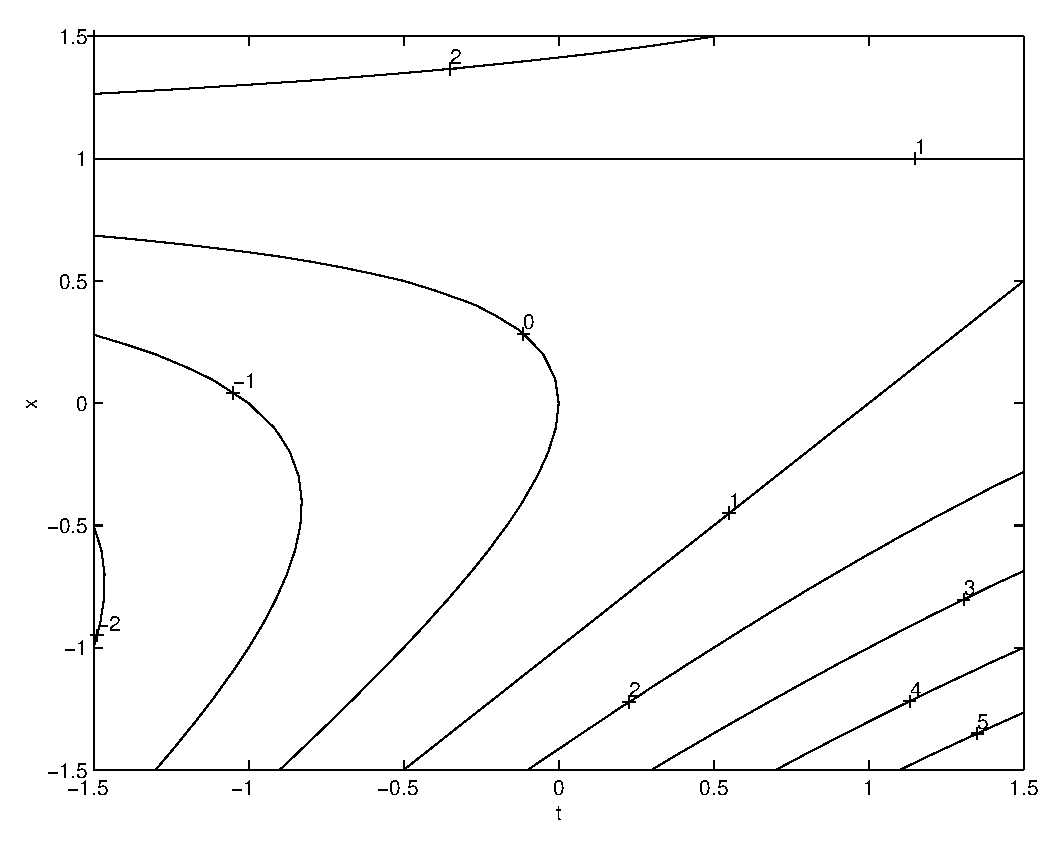
\psfig{file=figures/contour1.eps,width=3.5in}}
           \caption{Contour lines of $F(t,x)=x^2-xt+t$ for
          $(t,x)\in[-1.5,1.5]\times[-1.5,1.5]$.}
           \label{Fig:contour1}
\end{figure}

Note that the straight line solutions $x(t)=1$ and $x(t)=t-1$ 
correspond to the level set for $c=1$, as expected.  We can also
see from Figure~\ref{Fig:contour1} that the contour lines for
the levels $c=0,-1,-2$ have a turning point, that is, they
cannot be parameterized entirely by $t$.  

Setting $c=0$ in \Ref{E:twosolns} we find the expressions
\[
x_+(t) = \frac{1}{2}\left(t+\sqrt{t(t-4)}\right) \AND
x_-(t) = \frac{1}{2}\left(t-\sqrt{t(t-4)}\right).
\]
These functions are not real-valued for $t\in (0,4)$.  In
particular, they cannot correspond to solutions of
\Ref{eq:exactex1} for these values of $t$.  This provides
an explanation for the existence of the turning point at
$(t,x)=(0,0)$ and why the solutions $x_+(t)$ and $x_-(t)$
``collide'' at this point.

Finally, we use {\sf dfield5}\index{\computer!dfield5} to confirm our 
theoretical discussion.  We set the values in {\sf the display window}
as in Figure~\ref{Fig:contour1} and start the computation in 
\[
(t_0,x_0)=(-0.5,x_-(-0.5))=(-0.5,-1)
\]
using the {\sf Keyboard input}.  The result --- which is in good
agreement with the contour plot\index{contour!plot} --- is shown in
Figure~\ref{Fig:contour2}.  Observe that {\sf dfield5} will not 
stop the computation of the forward orbit on its own and one has to
use the {\sf Stop} button to stop the numerical solution.  The reason is
that the program encounters numerical difficulties approaching the turning
point $(0,0)$, since the right hand side of the differential equation is
not defined at $(0,0)$.

\begin{figure}[htb]
  \centerline{%
  \psfig{file=figures/contour2.eps,width=3.7in}}
  \caption{The solution of \protect\Ref{eq:exactex1} for the
  initial value $(t_0,x_0)=(-0.5,-1)$ computed by {\sf dfield5}.}
  \label{Fig:contour2}
\end{figure}

\subsection*{The General Definition of Exact Differential Equations}

After this motivating example, we consider the general
situation.  Suppose that we have an ordinary differential
equation of the form
\begin{equation} \label{eq:exact}
\frac{dx}{dt} = \frac{G(t,x)}{H(t,x)},
\end{equation}
where $G$ and $H$ are real-valued continuous functions.  In 
\Ref{eq:exactex1}, $G(t,x)=x-1$ and $H(t,x) = 2x-t$.
The differential equation \Ref{eq:exact} is {\em exact\/} 
\index{differential equation!exact} if
there is a function $F(t,x)$ such that
\begin{equation}  \label{e:FGH}
\frac{\partial F}{\partial t} = -G \AND
\frac{\partial F}{\partial x} =  H.
\end{equation}
Indeed, the differential equation \Ref{eq:exactex1} is exact --- just set 
$F(t,x) = x^2 - xt + t$.

Supposing that the differential equation \Ref{eq:exact} is exact, proceed as 
in the example by rewriting \Ref{eq:exact} as 
\begin{equation} \label{eq:exacta}
H(t,x)\frac{dx}{dt} - G(t,x) = 0.
\end{equation}
Let $x(t)$ be a solution to \Ref{eq:exactex1} and use the chain rule, 
\Ref{e:FGH}, and \Ref{eq:exacta} to obtain
\[
\frac{d}{dt} F(t,x(t)) = \frac{\partial F}{\partial x}\frac{dx}{dt} + 
\frac{\partial F}{\partial t} = H\frac{dx}{dt}-G = 0.
\]
Hence, solutions of \Ref{eq:exact} must lie on a level set of $F$ defined 
by $F(t,x) = c$. We have proved:

\begin{thm} \label{thm:exact}
Assume that the differential equation \Ref{eq:exact} is exact.  Then, for any 
solution $x(t)$ of \Ref{eq:exact} with $x(t_0)=x_0$, there is a constant $c$ 
such that for all $t$ close to $t_0$, $F(t,x(t)) = c$.
\end{thm}\index{differential equation!exact}

\subsection*{On the Existence of $F$}

In order to solve exact differential equations,
\index{differential equation!exact} we must answer two 
questions: 
\begin{itemize}
\item When does a function $F$ exist that satisfies the 
conditions in \Ref{e:FGH}?
\item If the function $F$ exists, then how can we compute it?
\end{itemize}
The following proposition, based on the equality of mixed partial derivatives, 
gives a necessary condition for having a positive answer to the first question.

\begin{prop} \label{prop:exact}
Let $G,H:\R^2\to\R$ be differentiable functions such that
$\partial G/\partial x$ and $\partial H/\partial t$ are
continuous.  Suppose that the corresponding differential
equation \Ref{eq:exact} is exact.  Then
\begin{equation} \label{eq:Gy=Hs}
-\frac{\partial G}{\partial x} (t,x) = \frac{\partial H}{\partial
t} (t,x).
\end{equation}
\end{prop}

\proof Using \Ref{e:FGH} we compute
\[
\frac{\partial^2 F}{\partial x\partial t} = 
-\frac{\partial G}{\partial x} (t,x) \AND 
\frac{\partial^2 F}{\partial t\partial x} = 
\frac{\partial H}{\partial t} (t,x).
\]
Since $\partial G/\partial x$ and $\partial H/\partial t$ are
continuous, equality of mixed partial derivatives holds, and
\[
-\frac{\partial G}{\partial x} = 
\frac{\partial^2 F}{\partial x\partial t} =
\frac{\partial^2 F}{\partial t\partial x} =
\frac{\partial H}{\partial t},
\]
as desired. \qed

\begin{rmk} \label{rmk:exact}
{\rm It can be shown that criterion \Ref{eq:Gy=Hs} is also
sufficient for the exactness of the corresponding differential
equation, if this criterion is satisfied in a region in the
$(t,x)$-plane having no holes. The proof of this result can be
found in any text on multidimensional calculus.}
\end{rmk}


\subsubsection*{Two Examples}

We use two examples to illustrate the test for exactness
\index{differential equation!exact!test for}
of the underlying differential equation given by \Ref{eq:Gy=Hs}.

\noindent (a) Consider \Ref{eq:exactex1}, that is, suppose $G(t,x)=x-1$ and 
$H(t,x)=2x-t$.  Then
\[
-\frac{\partial G}{\partial x} = -1 = 
\frac{\partial H}{\partial t},
\]
and according to Remark~\ref{rmk:exact} a function $F$ with the desired 
properties may be found.

\noindent (b) Suppose that $G(t,x) = 1$ and $H(t,x) = t$.  Then 
\[
-\frac{\partial G}{\partial x} (t,x) = 0\not= 1 = 
\frac{\partial H}{\partial t} (t,x),
\]
and by Proposition~\ref{prop:exact} a function $F$ satisfying \Ref{e:FGH} 
cannot exist.

\subsection*{On the Computation of $F$}
Next, consider the second question, namely, how can $F$ be
computed when it exists.  By \Ref{e:FGH} we have
\[
\frac{\partial F}{\partial t}(t,x) = -G(t,x).
\]
Therefore, there is a differentiable function $g:\R\to\R$ such
that
\begin{equation}  \label{eq:defGamma}
F(t,x) = -\Gamma(t,x) + g(x),
\end{equation}
where 
\[
\Gamma(t,x)=\int G(\tau,x) d\tau
\]
is an indefinite integral of $G$ with respect to the variable $t$.
Condition \Ref{e:FGH} also implies that
\[
H(t,x) = \frac{\partial F}{\partial x}(t,x) =
-\frac{\partial}{\partial x}\Gamma(t,x) + g'(x),
\]
that is
\begin{equation} \label{eq:defg}
g'(x) = \frac{\partial}{\partial x}\Gamma(t,x) + H(t,x).
\end{equation}
Equations \Ref{eq:defg} and \Ref{eq:defGamma} can now be used 
to compute the function $F$ as long as the corresponding
integrations can be performed.  

Equivalently, we can first integrate the condition $F_x=H$ to obtain
\begin{equation}  \label{eq:excond}
F(t,x) = \Omega(t,x) + h(t),
\end{equation}
where $\Omega(t,x)=\int H(t,x)dx$ is an indefinite integral of $H$ with
respect to $x$.  Then \Ref{e:FGH} leads to
\[
h'(t) = -\frac{\partial}{\partial t}\Omega(t,x) - G(t,x).
\]
In practice, we prefer one way to the other depending on which
integrations are easier to perform.

\subsubsection*{Two Examples}

\noindent (a) Reconsider \Ref{eq:exactex1}, that is, suppose $G(t,x)=x-1$ and 
$H(t,x)=2x-t$.  We can choose
\[
\Gamma(t,x)=\int G(\tau,y)d\tau = tx-t,
\]
and \Ref{eq:defg} becomes
\[
g'(x) = t + H(t,x) = 2x.
\]
We can then choose $g(x)=x^2$ and, by \Ref{eq:defGamma}, obtain
\[
F(t,x) = -\Gamma(t,x) + g(x) = -tx + t + x^2.
\]

\noindent (b) Next, consider the differential equation
\begin{equation}  \label{eq:exacex2}
\frac{dx}{dt} = \frac{2t(1-x^2)-x^6}{x(2t^2+3x+6tx^4)}.
\end{equation}
In our notation
\[
G(t,x) = 2t(1-x^2)-x^6 \AND H(t,x) = x(2t^2+3x+6tx^4).
\]
Therefore, 
\[
-\frac{\partial G}{\partial x} = 4tx + 6x^5 = 
\frac{\partial H}{\partial t}.
\]
Hence the equation is exact (see Proposition~\ref{prop:exact} and 
Remark~\ref{rmk:exact}).  

It is easier to compute $\Gamma(t,x)=\int G(\tau,x) d\tau$ than 
$\Omega(t,x)=\int H(s,x)dx$.  We choose 
\[
\Gamma(t,x) = t^2(1-x^2) - tx^6,
\]
and \Ref{eq:defg} becomes
\[
g'(x) = -(2t^2 x + 6tx^5) + x(2t^2+3x+6tx^4) = 3x^2.
\]
Now we use \Ref{eq:defGamma} to obtain
\[
F(t,x) = t^2(x^2-1) + tx^6 + x^3.
\]
Solutions of the differential equation \Ref{eq:exacex2} lie on
level sets of $F$.  In particular, the solution $x(t)$
determined by the initial condition $x(2)=1$ satisfies 
\[
F(t,x)=t^2(x^2-1) + tx^6 + x^3 = 3,
\]
since $F(2,1)=3$.  To see the qualitative behavior of the
solutions\index{contour!plot} we use the following sequence 
of \Matlab commands
\begin{verbatim}
[t,x] = meshgrid(1:0.02:3,0.5:0.01:1.5);
F  = t.^2.*(x.^2-1) + t.*x.^6 + x.^3;
cs = contour(t,x,F,[0,3,6,9,12]);
clabel(cs)
hold on
plot(2,1,'o')                  
xlabel('t')
ylabel('x')
\end{verbatim}\index{\computer!meshgrid}\index{\computer!contour}
\index{\computer!hold}\index{\computer!clabel}\index{\computer!plot}
The result is shown in Figure~\ref{Fig:contour3}.  

\begin{figure}[htb]
  \centerline{%
  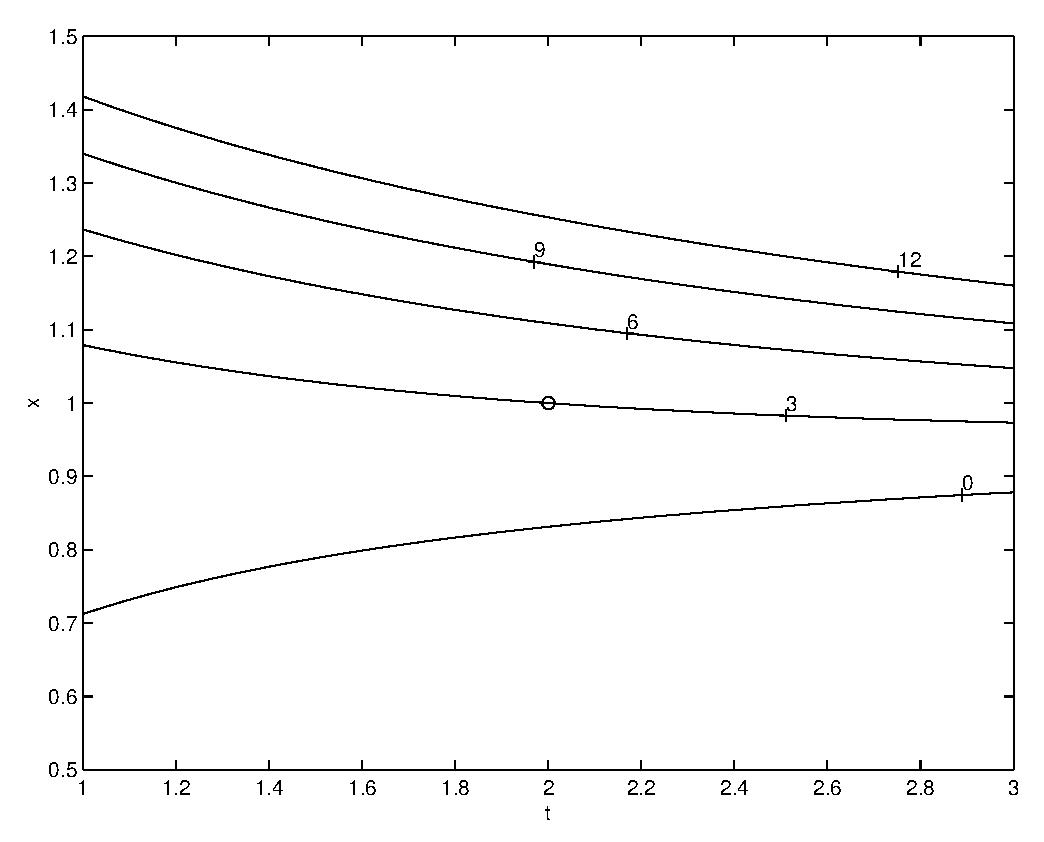
\psfig{file=figures/contour3.eps,width=3.5in}}
  \caption{Solutions of the differential equation
\protect\Ref{eq:exacex2}
  corresponding to the levels $c=0,3,6,9,12$ in the rectangle
  $[1,3]\times [0.5,1.5]$.}
\label{Fig:contour3}
\end{figure}


\EXER

\TEXER

\noindent In Exercises~\ref{c14.6.2} -- \ref{c14.6.3} determine whether or 
not the given differential equations is exact.
\begin{exercise} \label{c14.6.2}
$\dps \frac{dx}{dt} = \frac{\cos x}{t\sin x}$.
\end{exercise}
\begin{exercise} \label{c14.6.3}
$\dps \frac{dx}{dt} = \frac{\cos t}{x\sin t}$.
\end{exercise}

\begin{exercise} \label{c14.6.4}
Verify that the differential equation 
\[
\dps\frac{dx}{dt} = \dps \frac{2t-x}{t+1} 
\]
is exact and find a solution with initial value $x(0) = 3$.
\end{exercise}

\begin{exercise} \label{c14.6.6}
Verify that the differential equation 
\[
\frac{dx}{dt} = \frac{x}{x-t}
\]
is exact and find a solution with initial value $x(2)=3$.   Compare your 
answer with Exercise~\ref{exer:at} in Section~\ref{S:3.2}.
\end{exercise} 

\begin{exercise}  \label{ex:if}
Show that the differential equation
\begin{equation} \label{Ex:nexact}
\frac{dx}{dt} = -\frac{1+3tx}{t^2}
\end{equation}
is not exact.  Now multiply both the numerator and denominator of the 
right side of \Ref{Ex:nexact} by $t$ and show that this `new' differential
equation 
\[
\frac{dx}{dt} = -\frac{t+3t^2x}{t^3}
\]
is exact. Now find all solutions to \Ref{Ex:nexact}.
\end{exercise}

\begin{exercise}  \label{ex:if2}
Show that the differential equation
\begin{equation} \label{Ex:nexact2}
\frac{dx}{dt} = -\frac{3x}{2t}
\end{equation}
is not exact.  Now multiply both the numerator and denominator of the 
right side of \Ref{Ex:nexact2} by $t^2x$ and show that this `new' differential
equation 
\[
\frac{dx}{dt} = -\frac{3t^2x^2}{2t^3x}
\]
is exact.  Now find all solutions to \Ref{Ex:nexact2}.
\end{exercise}

\begin{exercise} \label{c14.6.7}
Let $G,H:\R^2\to\R$ be continuous functions and suppose that the differential 
equation 
\begin{equation}  \label{eq:if1}
\frac{dx}{dt} = \frac{G(t,x)}{H(t,x)}
\end{equation}
is {\bf not} exact.   An {\em integrating factor\/} for \Ref{eq:if1} is 
a function $\rho:\R^2\rightarrow\R$ such that the differential equation
\[
\frac{dx}{dt} = \frac{\rho(t,x) G(t,x)}{\rho(t,x)H(t,x)}
\]
is exact.  Suppose that there exists an integrating factor $\rho(t)$ for 
\Ref{eq:if1} that is a function of $t$ alone.  Show that $\rho$ satisfies
\[
\frac{d\rho}{dt} = -\frac{\rho}{H}
\left( \frac{\partial G}{\partial x}+\frac{\partial H}{\partial t}\right).
\]
\end{exercise}

\begin{exercise} \label{c14.6.7A}
Use the result of Exercise~\ref{c14.6.7} to find an integrating factor for 
the differential equation
\[
\frac{dx}{dt} = -\frac{8x+5t}{4t},
\]
and then determine all solutions of this differential equation.
\end{exercise}

\CEXER


\begin{exercise} \label{c14.6.8}
Consider the differential equation
\[
\frac{dx}{dt} = -\frac{2tx+\cos x}{t(t-\sin x)}.
\]
Show that this differential equation is 
exact.  Then use the command {\tt contour}\index{\computer!contour} in \Matlab 
to find solutions.  For the display, 
use the rectangle $[-2,2]\times [-2,2]$ in the $(t,x)$-plane and show contour
lines for the different levels $c=-4,-3,-2,-1,0,1,2,3,4$.  Mark the solution
which satisfies the initial condition $x(1)=0$ by a circle.
{\bf Hint:} Use the same procedure that was used to create 
Figure~\ref{Fig:contour3}.
\end{exercise}


\Section{Hamiltonian Systems}
\label{sec:HamSys}
\index{Hamiltonian system}

In the previous sections we have considered solution techniques that
can be applied to {\em scalar\/} differential equations.  In this section 
we present {\em planar\/} ODEs of a specific structure for which 
--- similar to the case of exact differential equations, see 
Section~\ref{S:exact} --- solutions
can be identified as level curves of a certain function.

An autonomous\index{autonomous} planar system of differential equations 
\begin{equation}  \label{e:ham}
\begin{array}{rcl} 
\dot{x} & = & f(x,y) \\
\dot{y} & = & g(x,y) 
\end{array}
\end{equation}
is {\em Hamiltonian\/}\index{Hamiltonian system} if there exists a real-valued
function $H(x,y)$ such that 
\[
f(x,y) = \frac{\partial H}{\partial y}(x,y) \AND 
g(x,y) =-\frac{\partial H}{\partial x}(x,y).
\]
The function $H$ is called the {\em Hamiltonian\/}\index{Hamiltonian system}
of the system \Ref{e:ham}.
By the following result Hamiltonian systems can be solved in a way analogous 
to exact systems.

\begin{thm}
Every solution trajectory of the Hamiltonian system \Ref{e:ham} lies
on a level curve\index{level curve} of the associated Hamiltonian $H$.
\end{thm}

\proof 
Let $(x(t),y(t))$ be a solution trajectory of \Ref{e:ham}.  We need to 
verify that $H(x(t),y(t))$ is constant in $t$.  This is most easily 
accomplished by showing that 
\begin{equation} \label{e:dH=0}
\frac{d}{dt} H(x(t),y(t)) = 0.
\end{equation}
Evaluate the left hand side of \Ref{e:dH=0} by using the chain rule:
\begin{eqnarray*}
\frac{d}{dt} H(x(t),y(t)) & = & \frac{\partial H}{\partial x}\frac{dx}{dt}
+ \frac{\partial H}{\partial y} \frac{dy}{dt} \\
& = & -g\frac{dx}{dt} + f\frac{dy}{dt}, 
\end{eqnarray*}
where the last equality follows from the definition of the Hamiltonian.  
Using the fact that $(x(t),y(t))$ is a solution of \Ref{e:ham} leads to 
\[
 \frac{d}{dt} H(x(t),y(t)) = -gf+fg = 0,
\]
as desired.  \qed

\subsection*{Potential Systems}
\index{potential!system}
The system of differential equations
\begin{equation}  \label{e:hamex}
\begin{array}{rcl} 
\dot{x} & = & y \\
\dot{y} & = & -V'(x) 
\end{array}
\end{equation}
is a Hamiltonian system for any {\em potential\/} function $V(x)$,
\index{potential!function}
where the Hamiltonian\index{Hamiltonian system} is
\[
H(x,y) = \frac{1}{2}y^2 + V(x).
\]
To verify this point, just check that 
\[
-\frac{\partial H}{\partial x} = -V'(x) \AND \frac{\partial H}{\partial y} = y.
\]

In particular, the linear center\index{center} is a 
Hamiltonian system\index{Hamiltonian system}; just take 
$V(x)=\frac{1}{2}x^2$ so that 
\[
H(x,y) = \frac{1}{2}(x^2+y^2).
\]
Note that the level curves of this Hamiltonian are just circles centered 
at the origin.  This observation provides a second verification that 
trajectories of this center lie on circles.

A more interesting example occurs if we take the potential function 
equal to 
\[
V(x) = \frac{1}{4}x^4 - \frac{1}{2}x^2.
\]
The corresponding Hamiltonian system is:
\begin{equation*}  \label{e:hamex1}
\begin{array}{rcl} 
\dot{x} & = & y \\
\dot{y} & = & x-x^3 
\end{array}
\end{equation*}%
since $V'(x)=x^3-x$.  It is easy to verify that \Ref{e:hamex1} has three 
equilibria at $(1,0)$, $(0,0)$, and $(-1,0)$.  

The Jacobian of \Ref{e:hamex} is
\[
J = \left(\begin{array}{cc}  0 & 1 \\ -V''(x) & 0 \end{array}\right).
\]
Thus equilibria of \Ref{e:hamex} are saddles\index{saddle} 
if $V''<0$ or centers if $V''>0$.
Indeed, this dichotomy is generally valid for Hamiltonian systems and 
Hamiltonian systems are {\em not\/} usually Morse-Smale.  For instance, in
\Ref{e:hamex1} 
\[
V''(x) = 3x^2-1
\]
and the origin is a saddle while the other two equilibria are centers. 

For planar Hamiltonian systems, it is always the case (this is a theorem
similar to the Hopf bifurcation theorem) that centers are surrounded by 
a continuous family of periodic 
trajectories\index{family of periodic solutions}.  Using 
{\sf pplane5}\index{\computer!pplane5} we can
compute the phase portrait\index{phase!portrait} for 
this potential system\index{potential!system} and verify the 
existence of continuous families of periodic trajectories.  The result 
is presented in Figure~\ref{F:hamex}.  Note the numerical evidence for 
the existence of two homoclinic trajectories\index{trajectory!homoclinic}.  
\begin{figure}[htb]
           \centerline{%
	   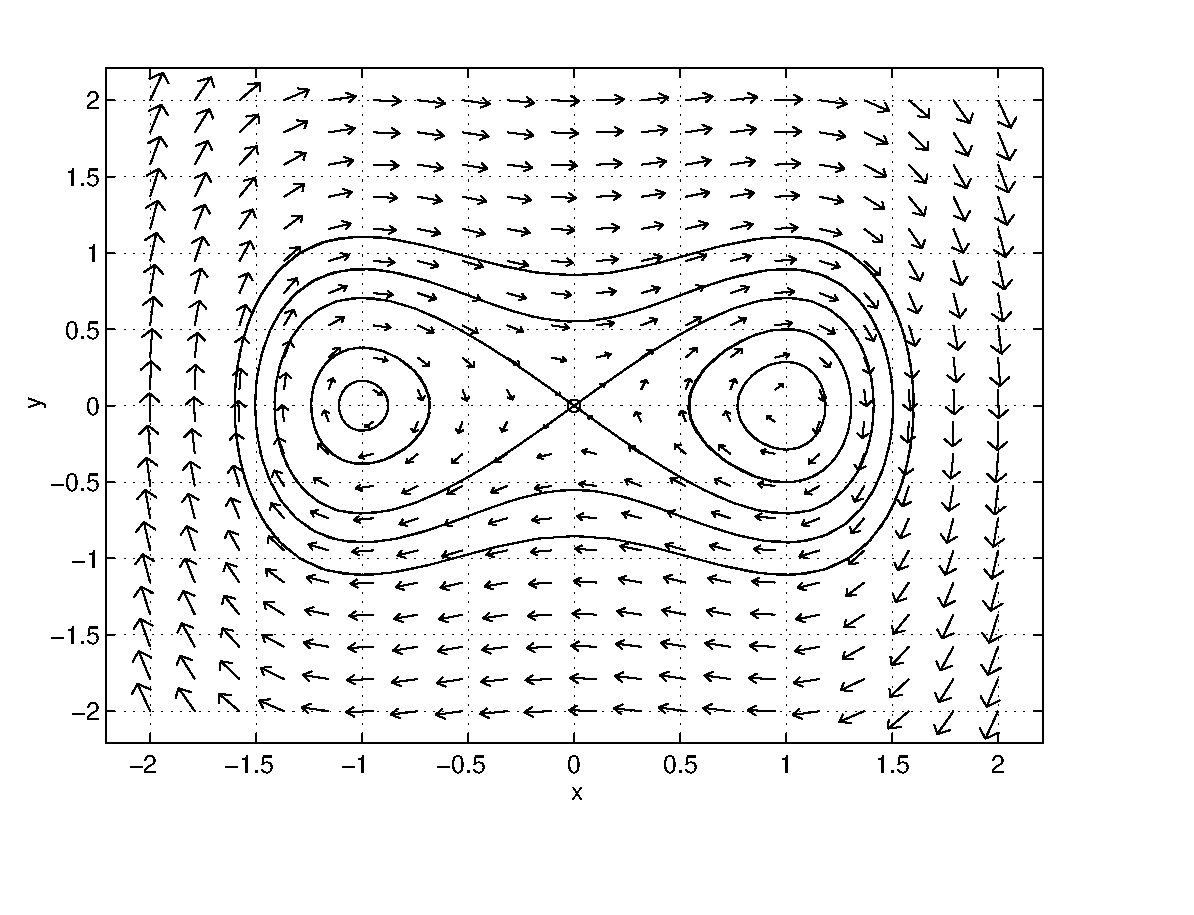
\psfig{file=figures/ham.eps,width=3.5in}}
           \caption{Phase portrait of \protect\Ref{e:hamex1}}
           \label{F:hamex}
\end{figure}

We remark that the system \Ref{e:hamex} is just the one obtained from the 
second order equation 
\begin{equation}  \label{e:V(x)}
\ddot{x} + V(x) = 0
\end{equation}
by the trick of setting $y=\dot{x}$ to obtain a planar system. 

\subsection*{Newton's Second Law and Potential Systems}
\index{potential!system}

There are several related interpretations of the potential $V$ in
\Ref{e:hamex} all based on Newton's second law of motion. 
\index{Newton's second law}  In particular, we can rewrite \Ref{e:V(x)} as 
\[
\ddot{x} =  -V(x)
\]
and interpret $-V$ as the force acting on a 
particle\index{particle motion} of unit mass\index{mass}.  In this 
interpretation it is assumed that the force just depends on the value of $x$. 

We consider three examples.
\begin{itemize}
\item[(a)] Suppose that $x$ is the position of a unit mass on a vertical 
line moving under the influence of gravity.  Then $V(x)=g$, where 
$g$ is the gravitational constant.
\item[(b)] Suppose that $x$ is the distance of a particle of unit mass from 
the sun.  The gravitational attraction of the sun is given by the inverse
square law. Assuming that the sun is at the origin, $V(x)= \frac{1}{x^2}$.
\item[(c)] Consider a pendulum\index{pendulum} 
with a unit mass attached to its end.  Assume, 
that the pendulum itself is idealized to have unit length and zero mass.  
The motion of an ideal pendulum is driven only by gravity. To derive the 
force acting on the pendulum, let $x$ be the angle that the pendulum makes 
with the vertical, as in Figure~\ref{F:pendulum}.  In that figure, the angle
$z=\frac{\pi}{2}-x$.  Then the force on the pendulum is $g\cos z=g\sin x$ 
and the pendulum equation is:
\begin{equation*} \label{e:pendulum}
\begin{array}{rcl} 
\dot{x} & = & y \\
\dot{y} & = & -g\sin x. 
\end{array}
\end{equation*}
\end{itemize}
\begin{figure}[htb]
           \centerline{%
	   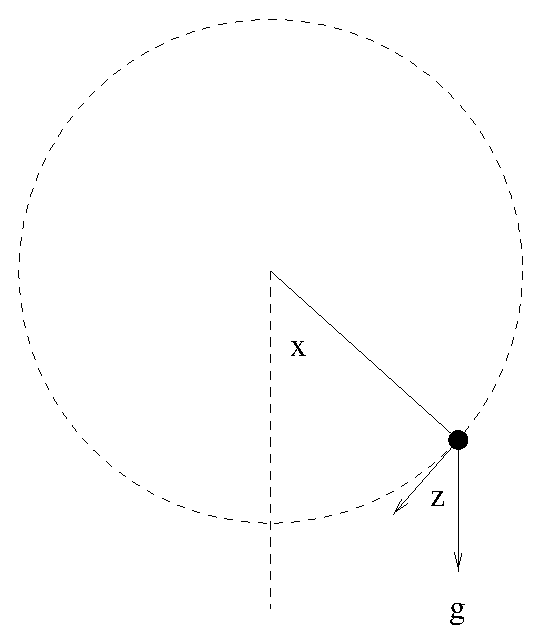
\psfig{file=figures/pendulum.eps,width=2.0in}}
           \caption{Pendulum geometry}
           \label{F:pendulum}
\end{figure}
The phase portrait for the pendulum equations is shown in Figure~\ref{F:ppen}.
\begin{figure}[htb]
           \centerline{%
	   \psfig{file=figures/ppen.eps,width=3.5in}}
           \caption{Phase portrait of the pendulum equation 
		\protect\Ref{e:pendulum}}
           \label{F:ppen}
\end{figure}


\subsubsection*{The Two Body Problem}

As a final example, consider the motion of two bodies of masses $m_1$ and 
$m_2$ under the influence of an attractive inverse square law of force.  Both 
bodies move in three dimensional space and therefore their motion would in 
principle be described by a system of three second order ODEs. However, by 
considering the motion inside an appropriate moving frame it is possible to 
neglect both the translational motion in space and the rotation of the two 
bodies around their common center of mass.  If this is done then the relative 
motion of the two bodies is described by the single second order equation
\begin{equation} \label{E:2body}
m\ddot x = -\frac{1}{x^2} + \frac{\ell^2}{mx^3}.
\end{equation}
Here $x(t)$ is the distance between the two bodies at time $t$,  $\ell$ is 
the (constant) {\em angular momentum\/} related to their rotational motion, 
and $m=m_1 m_2/(m_1 + m_2)$ is the {\em reduced mass}. 
We can rewrite \Ref{E:2body} in the form $\ddot{x}+V(x)=0$ where
\[
V(x) =  \frac{1}{mx^2} - \frac{\ell^2}{m^2x^3}.
\]
For two unit masses $m_1=m_2=1$ (that is, $m=1/2$) with angular momentum 
$\ell = 1$, we can rewrite the second order equation as the first order system 
\begin{equation*} \label{e:tbp}
\begin{array}{rcl}
\dot{x} & = & y \\
\dot{y} & = & -\frac{2}{x^2} + \frac{4}{x^3}.
\end{array}
\end{equation*}
The phase portrait of \Ref{e:tbp} is shown in Figure~\ref{fig:tbp}.  In 
physical space, the steady-state solution $(x,y)=(2,0)$ corresponds to a 
circular motion of the two bodies around their common center of mass and 
the periodic solutions correspond to motions on ellipsoids.

\begin{figure}[htb]
           \centerline{%
           \psfig{file=figures/tbp.eps,height=2.5in}}
           \caption{Phase portrait of the equation
                \protect\Ref{e:tbp}}
           \label{fig:tbp}
\end{figure}



\EXER

\TEXER

%\begin{exercise}
%Let $V(x) = x-x^3$.  Verify that the potential system \Ref{e:hamex} has
%three equilibria at the origin and at $(\pm 1,0)$.  Show that the origin 
%is a center and that the other equilibria are saddles.  Use {\sf pplane5}
%to find the phase portrait of this system.  How many heteroclinic 
%trajectories are there in this Hamiltonian system?
%\end{exercise}

\noindent In Exercises~\ref{c14.7.1} -- \ref{c14.7.4} write the system of 
differential equations corresponding to each of the given Hamiltonians. 
\begin{exercise} \label{c14.7.1}
$H(x,y) = x+3y+2$.
\end{exercise}
\begin{exercise} \label{c14.7.2}
$H(x,y) = y^3$.
\end{exercise}
\begin{exercise} \label{c14.7.3}
$H(x,y) = 1 + \sin x \cos y$.
\end{exercise}
\begin{exercise} \label{c14.7.4}
$H(x,y) = xy^2 - x + x\cos y$.
\end{exercise}

\noindent In Exercises~\ref{c14.7.5} -- \ref{c14.7.7} decide whether or not  
the given planar systems of differential equations is Hamiltonian:
\begin{exercise} \label{c14.7.5}
$\begin{array}{rcl}
\dot{x} & = & 0 \\
\dot{y} & = & -1.
\end{array}$
\end{exercise}
\begin{exercise} \label{c14.7.6}
$\begin{array}{rcl}
\dot{x} & = & x\\
\dot{y} & = & y.
\end{array}$
\end{exercise}
\begin{exercise} \label{c14.7.6a}
$\begin{array}{rcl}
\dot{x} & = & x - y^2\\
\dot{y} & = & -y - x^2.
\end{array}$
\end{exercise}
\begin{exercise} \label{c14.7.7}
$\begin{array}{rcl}
\dot{x} & = & x\cos y\\
\dot{y} & = & -\sin y.
\end{array}$
\end{exercise}

\begin{exercise} \label{c14.7.8}
Let $J$ be the Jacobian matrix of an equilibrium in a planar Hamiltonian 
system. Show that $\trace(J)=0$.  If $\det(J)\neq 0$, what are the possible
types for this equilibrium?
\end{exercise}

\begin{exercise} \label{c14.7.9}
Determine the equilibria in the pendulum equations \Ref{e:pendulum}.
Refer to the phase portrait of the ideal pendulum in Figure~\ref{F:ppen}
and describe in words the motion of the pendulum corresponding to a periodic 
solution surrounding one of the centers.  Describe the motion of the 
pendulum corresponding to the initial condition $(x(0),y(0))=(0,2)$.
\end{exercise}

\begin{exercise} \label{c14.7.10}
Consider the Hamiltonian  $H(x,y) = x^3 + x^2 - y^2$.  Show that the 
associated Hamiltonian system has a homoclinic trajectory.  {\bf Hint:} 
Consider the level curve $H(x,y)=0$.\index{homoclinic}
\end{exercise}

\begin{exercise} \label{c14.7.11} 
Consider the Hamiltonian  $H(x,y) = -\frac{1}{4}x^4 + \frac{1}{2}x^2 + y^2$.  
Show that the associated Hamiltonian system has saddle points at $(\pm 1,0)$ 
and heteroclinic trajectories connecting these saddle points.  {\bf Hint:} 
Consider the level curve $H(x,y) = \frac{1}{4}$.\index{heteroclinic}
\end{exercise}






 





